% Options for packages loaded elsewhere
\PassOptionsToPackage{unicode}{hyperref}
\PassOptionsToPackage{hyphens}{url}
\PassOptionsToPackage{dvipsnames,svgnames,x11names}{xcolor}
%
\documentclass[
  sn-nature,
  11pt,
]{sn-jnl}



\usepackage{amsmath,amssymb}
\usepackage{iftex}
\ifPDFTeX
  \usepackage[T1]{fontenc}
  \usepackage[utf8]{inputenc}
  \usepackage{textcomp} % provide euro and other symbols
\else % if luatex or xetex
  \usepackage{unicode-math}
  \defaultfontfeatures{Scale=MatchLowercase}
  \defaultfontfeatures[\rmfamily]{Ligatures=TeX,Scale=1}
\fi
\usepackage{lmodern}
\ifPDFTeX\else  
    % xetex/luatex font selection
\fi
% Use upquote if available, for straight quotes in verbatim environments
\IfFileExists{upquote.sty}{\usepackage{upquote}}{}
\IfFileExists{microtype.sty}{% use microtype if available
  \usepackage[]{microtype}
  \UseMicrotypeSet[protrusion]{basicmath} % disable protrusion for tt fonts
}{}
\makeatletter
\@ifundefined{KOMAClassName}{% if non-KOMA class
  \IfFileExists{parskip.sty}{%
    \usepackage{parskip}
  }{% else
    \setlength{\parindent}{0pt}
    \setlength{\parskip}{6pt plus 2pt minus 1pt}}
}{% if KOMA class
  \KOMAoptions{parskip=half}}
\makeatother
\usepackage{xcolor}
\setlength{\emergencystretch}{3em} % prevent overfull lines
\setcounter{secnumdepth}{-\maxdimen} % remove section numbering
% Make \paragraph and \subparagraph free-standing
\makeatletter
\ifx\paragraph\undefined\else
  \let\oldparagraph\paragraph
  \renewcommand{\paragraph}{
    \@ifstar
      \xxxParagraphStar
      \xxxParagraphNoStar
  }
  \newcommand{\xxxParagraphStar}[1]{\oldparagraph*{#1}\mbox{}}
  \newcommand{\xxxParagraphNoStar}[1]{\oldparagraph{#1}\mbox{}}
\fi
\ifx\subparagraph\undefined\else
  \let\oldsubparagraph\subparagraph
  \renewcommand{\subparagraph}{
    \@ifstar
      \xxxSubParagraphStar
      \xxxSubParagraphNoStar
  }
  \newcommand{\xxxSubParagraphStar}[1]{\oldsubparagraph*{#1}\mbox{}}
  \newcommand{\xxxSubParagraphNoStar}[1]{\oldsubparagraph{#1}\mbox{}}
\fi
\makeatother


\providecommand{\tightlist}{%
  \setlength{\itemsep}{0pt}\setlength{\parskip}{0pt}}\usepackage{longtable,booktabs,array}
\usepackage{calc} % for calculating minipage widths
% Correct order of tables after \paragraph or \subparagraph
\usepackage{etoolbox}
\makeatletter
\patchcmd\longtable{\par}{\if@noskipsec\mbox{}\fi\par}{}{}
\makeatother
% Allow footnotes in longtable head/foot
\IfFileExists{footnotehyper.sty}{\usepackage{footnotehyper}}{\usepackage{footnote}}
\makesavenoteenv{longtable}
\usepackage{graphicx}
\makeatletter
\newsavebox\pandoc@box
\newcommand*\pandocbounded[1]{% scales image to fit in text height/width
  \sbox\pandoc@box{#1}%
  \Gscale@div\@tempa{\textheight}{\dimexpr\ht\pandoc@box+\dp\pandoc@box\relax}%
  \Gscale@div\@tempb{\linewidth}{\wd\pandoc@box}%
  \ifdim\@tempb\p@<\@tempa\p@\let\@tempa\@tempb\fi% select the smaller of both
  \ifdim\@tempa\p@<\p@\scalebox{\@tempa}{\usebox\pandoc@box}%
  \else\usebox{\pandoc@box}%
  \fi%
}
% Set default figure placement to htbp
\def\fps@figure{htbp}
\makeatother
% definitions for citeproc citations
\NewDocumentCommand\citeproctext{}{}
\NewDocumentCommand\citeproc{mm}{%
  \begingroup\def\citeproctext{#2}\cite{#1}\endgroup}
\makeatletter
 % allow citations to break across lines
 \let\@cite@ofmt\@firstofone
 % avoid brackets around text for \cite:
 \def\@biblabel#1{}
 \def\@cite#1#2{{#1\if@tempswa , #2\fi}}
\makeatother
\newlength{\cslhangindent}
\setlength{\cslhangindent}{1.5em}
\newlength{\csllabelwidth}
\setlength{\csllabelwidth}{3em}
\newenvironment{CSLReferences}[2] % #1 hanging-indent, #2 entry-spacing
 {\begin{list}{}{%
  \setlength{\itemindent}{0pt}
  \setlength{\leftmargin}{0pt}
  \setlength{\parsep}{0pt}
  % turn on hanging indent if param 1 is 1
  \ifodd #1
   \setlength{\leftmargin}{\cslhangindent}
   \setlength{\itemindent}{-1\cslhangindent}
  \fi
  % set entry spacing
  \setlength{\itemsep}{#2\baselineskip}}}
 {\end{list}}
\usepackage{calc}
\newcommand{\CSLBlock}[1]{\hfill\break\parbox[t]{\linewidth}{\strut\ignorespaces#1\strut}}
\newcommand{\CSLLeftMargin}[1]{\parbox[t]{\csllabelwidth}{\strut#1\strut}}
\newcommand{\CSLRightInline}[1]{\parbox[t]{\linewidth - \csllabelwidth}{\strut#1\strut}}
\newcommand{\CSLIndent}[1]{\hspace{\cslhangindent}#1}

%%%% Standard Packages

\usepackage{graphicx}%
\usepackage{multirow}%
\usepackage{amsmath,amssymb,amsfonts}%
\usepackage{amsthm}%
\usepackage{mathrsfs}%
\usepackage[title]{appendix}%
\usepackage{xcolor}%
\usepackage{textcomp}%
\usepackage{manyfoot}%
\usepackage{booktabs}%
\usepackage{algorithm}%
\usepackage{algorithmicx}%
\usepackage{algpseudocode}%
\usepackage{listings}%

%%%%

\raggedbottom
\usepackage{lipsum} \usepackage{libertine} \usepackage[nolists,nomarkers]{endfloat}
\makeatletter
\@ifpackageloaded{caption}{}{\usepackage{caption}}
\AtBeginDocument{%
\ifdefined\contentsname
  \renewcommand*\contentsname{Table of contents}
\else
  \newcommand\contentsname{Table of contents}
\fi
\ifdefined\listfigurename
  \renewcommand*\listfigurename{List of Figures}
\else
  \newcommand\listfigurename{List of Figures}
\fi
\ifdefined\listtablename
  \renewcommand*\listtablename{List of Tables}
\else
  \newcommand\listtablename{List of Tables}
\fi
\ifdefined\figurename
  \renewcommand*\figurename{Figure}
\else
  \newcommand\figurename{Figure}
\fi
\ifdefined\tablename
  \renewcommand*\tablename{Table}
\else
  \newcommand\tablename{Table}
\fi
}
\@ifpackageloaded{float}{}{\usepackage{float}}
\floatstyle{ruled}
\@ifundefined{c@chapter}{\newfloat{codelisting}{h}{lop}}{\newfloat{codelisting}{h}{lop}[chapter]}
\floatname{codelisting}{Listing}
\newcommand*\listoflistings{\listof{codelisting}{List of Listings}}
\makeatother
\makeatletter
\makeatother
\makeatletter
\@ifpackageloaded{caption}{}{\usepackage{caption}}
\@ifpackageloaded{subcaption}{}{\usepackage{subcaption}}
\makeatother

\usepackage{bookmark}

\IfFileExists{xurl.sty}{\usepackage{xurl}}{} % add URL line breaks if available
\urlstyle{same} % disable monospaced font for URLs
\hypersetup{
  pdftitle={Estimating internal displacement in Ukraine from high-frequency GPS mobile phone data},
  pdfauthor={Rodgers Iradukunda; Francisco Rowe; Elisabetta Pietrostefani},
  pdfkeywords={internal population displacement, GSP mobile phone
data, Ukraine, disasters, climate, epidemics, conflict},
  colorlinks=true,
  linkcolor={blue},
  filecolor={Maroon},
  citecolor={Blue},
  urlcolor={Blue},
  pdfcreator={LaTeX via pandoc}}


\title[\textbf{Estimating internal displacement in Ukraine from
high-frequency GPS mobile phone data}]{\textbf{Estimating internal
displacement in Ukraine from high-frequency GPS mobile phone data}}

% author setup
\author[1]{\fnm{Rodgers} \sur{Iradukunda}}\author*[1]{\fnm{Francisco} \sur{Rowe}}\email{f.rowe-gonzalez@liverpool.ac.uk}\author[1]{\fnm{Elisabetta} \sur{Pietrostefani}}
% affil setup
\affil[1]{\orgdiv{Geographic Data Science Lab, Department of Geography
and Planning}, \orgname{University of Liverpool, Liverpool}}

% abstract 

\abstract{Nearly 110 million people are forcibly displaced people
worldwide. However, estimating the scale and patterns of internally
displaced persons in real time, and developing appropriate policy
responses, are hindered by traditional data streams because they are
infrequently updated, costly and slow. Mobile phone location data can
overcome these limitations, but only represent a population segment.
Drawing on an unprecedently large, high-frequency anonymised dataset of
locations from 25 million mobile devices, we develop a novel
methodological framework to leverage mobile phone data and produce
population-level estimates of internal displacement. We use this
framework to quantify the extent, pace and geographic patterns of
internal displacement in Ukraine during the early stages of the Russian
invasion in 2022. Our results produce validated population-level
estimates, enabling real-time monitoring of internal displacement at
detailed spatio-temporal resolutions (e.g.~daily, small administrative
units). The accurate estimations we provide are crucial in delivering
timely and effective humanitarian and disaster management responses,
prioritising resources where they are most needed. Given access to
similar mobile phone data, our methodology can be applied to estimating
population displacement in any geographical context globally in
situations of humanitarian crisis, namely climate-induced hazards,
conflict and epidemics.}

% keywords
\keywords{internal population displacement,  GSP mobile phone
data,  Ukraine,  disasters,  climate,  epidemics,  conflict}

\begin{document}
\maketitle


\newpage

The forced displacement of individuals, including refugees,
asylum-seekers and internally displaced people (IDP), creates
considerable humanitarian, social and economic costs (Blattman and
Miguel 2010; UNHCR 2022). Recent estimates indicates that the number of
forcibly displaced populations has significantly grown as result of
persecution, conflict, violence, human rights violations and disasters
(IDMC 2024). As of June 2023, the United Nations High Commissioner for
Refugees (UNHCR) estimated 110 million of forcibly displaced people
worldwide, with the number of IDP (62.5 million) accounting for the
largest share of these displacements (UNHCR 2023). The Russian
full-scale invasion of Ukraine is estimated to have created the fastest
global displacement crisis, and one of the largest, since the Second
World War (UNHCR 2022).

Forcibly displaced population data are key to inform operational plans,
humanitarian responses and long-term policy making. By understanding the
scale and locations where people are forcibly fleeing and the extent of
their return, government agencies, aid organisations and local community
groups can better prioritise and allocate resources and services where
they are most needed in the required quantities (IDMC 2024). Highly
granular geographical data tracking population displacements in real
time are therefore critical to support these efforts (Rowe 2022;
González-Leonardo et al. 2024).

Traditional data systems are constrained to render information at such
high temporal and geographical resolution and speed. Over the years,
UNHCR and the Internal Displacement Monitoring Centre (IDMC) have made
significant efforts triangulating various data sources to improve and
deliver global databases that enable the monitoring and management of
forced population displacements (IDMC 2024). However, they have also
identified persistent challenges in the production of reliable estimates
of forcibly displaced populations (Sarzin 2017; Tai, Mehra, and
Blumenstock 2022). Traditional data systems are not regularly updated,
costly and characterised by slow data collection and release (Rowe
2023). Particularly in conflict areas, humanitarian partners and data
collectors often face access restrictions due to violence and insecurity
preventing data gathering (UNHCR 2023). Data streams may also have gaps
collecting data on displacement during short-term evacuations or
spontaneous movements resulting from conflict and violence (Salah et al.
2019; Drouhot et al. 2022). The danger and challenging nature of field
work in conflict zones can also disrupt continuous engagement in data
collection by humanitarian and development agencies (Hoglund and Oberg
2011; Salehyan 2015).

Novel digital footprint data have emerged as a key source of information
offering an opportunity to capture human population movements at highly
granular geographical and temporal scales (Checchi et al. 2013; Rowe
2023; Spyratos et al. 2019). These data are automatically and
continuously generated avoiding exposure of data collectors to hazardous
areas and minimising potential data gaps (Salah et al. 2019). Mobile
phone location data have increasingly been used to monitor population
movements during crises, particularly measuring exposure to ambient
pollutant exposure (Nyhan et al. 2016; Dewulf et al. 2016), transport
patterns (Huang, Cheng, and Weibel 2019), recreational behaviour (Kim,
Kubo, and Nishihiro 2023), disaster-induced displacement (e.g.~flooding
and earthquakes) (Lu et al. 2016) and the spread of diseases - notably
during the COVID-19 pandemic (Kyra H. Grantz et al. 2020b; Finazzi
2023). Yet, limited work has been undertaken to estimate the scale and
patterns of IDP using mobile phone data.

Additionally, differences in the access and use of mobile phone
technology and applications used to collect location data prevent the
production of reliable population-level mobility estimates. Most
existing work based on mobile phone data has thus constrained to offer
rough signals about population movements (e.g.~spatial concentration),
trends (e.g.~increasing) and changes (e.g.~low to high) (Rowe 2023). For
example, a recent study (Shibuya, Jones, and Sekimoto 2024) used GPS
data to offer a granular representation of the geographic and temporal
patterns and trends in population displacement in Ukraine, but the
reported estimates correspond changes in the number of unique mobile
phone devices. They do not represent population-level figures. Estimates
need to be adjusted for biases to make them representative of the full
population.

To address these gaps, we propose an approach to produce high-frequency
population-level estimates of internal displacement drawing on location
data from 25 million unique devices. Our approach adapts Leasure's et
al.~approach (Leasure et al. 2023) of bias data correction to GPS human
mobility data. Leasure's et al.~developed a method of bias data
correction for Facebook users data extracted from Facebook Marketing
Advertising platform to produce estimates of population displacement in
Ukraine. A key limitation is that the Facebook Marketing Advertising
data represent counts of active Facebook users in an area at coarse
geographical scales. Thus, while they can be used to generate estimates
of local population counts, they do not allow the estimation of
displacement flows to identify displacement routes, their origins and
destinations, limiting their insights to support humanitarian
operations. Rather than as a simple application, we see the adaptation
of Leasure's et al.~approach to GPS data as a major extension of the
approach. It requires the engineering of raw GPS data (only containing a
device identifier, a timestamp, longitude and latitude) to identify home
locations before and after the start of the war, and then determine
changes in usual place of residence.

We make two substantive contributions. Our first contribution is
methodological and illustrates how high-frequency footprint data can
enable the generation of population-level estimates of internal
displacement correcting for differences in mobile phone-derived and
actual population counts, moving beyond providing rough signals. Most
prior work leveraging on digital footprint data to estimate population
displacement relies on social media or call detail records, with
location being inferred resulting in reduced precision (Ranjan et al.
2012; Zhao et al. 2016; Pestre, Letouzé, and Zagheni 2019). We use data
collected via GPS technology which provides greater precision data on
location (Kyra H. Grantz et al. 2020a).

Our second contribution is to provide evidence of the scale and spatial
patterns of population displacement in Ukraine during the first year of
the invasion. The Russian full-scale invasion of Ukraine has created the
fastest global displacement crisis, and one of the largest, since the
Second World War (UNHCR 2022). Recent estimates suggest that nearly
one-third of Ukrainian residents are estimated to have been forced from
their homes (UNHCR 2022). As of 25 September 2023, 3.67 million people
were estimated to have been displaced internally within Ukrainian
borders (IOM 2022b). These estimates are based on a random digit dial
telephone survey aiming at generating a nationally representative sample
of 2,000 individuals at each monthly round (IOM 2022b). While consistent
with high frequency estimates based on Facebook data (Leasure et al.
2023), these estimates cannot deliver population-level estimates of
population displacement for subnational areas at high granularity, or
high-temporal frequency. Our approach offers high frequency population
displacement estimates to complement data derived from traditional data
streams.

\section{Results}\label{results}

\subsection{Estimating the extent of internal population
displacement}\label{estimating-the-extent-of-internal-population-displacement}

We first estimate the extent of daily internal population displacement
at the oblast and raion level (Figure~\ref{fig-popdisplacement}). In
Ukraine, an oblast is the main first-level administrative division,
analogous to a state or region. Each oblast is further subdivided into
raions (districts), which are the second-level administrative units. As
a result of administrative reforms in 2020, Ukraine is currently divided
into 24 oblasts and 136 raions (including those in Crimea). Raions are
responsible for local governance and service delivery within their
boundaries, while oblasts serve as broader regional jurisdictions. We
estimate that over 5 million people were internally displaced from their
oblast of residence by April 2022 reaching an average of about 10
million in late July and August 2022. Figure~\ref{fig-popdisplacement}
reveals a drop in population displacement during mid-June and mid-July,
coinciding with a pattern of return displacements primarily to the
cities of Kiev and Kharkhiv (see Section on return movements). In
addition to return movements, subsequently higher but fluctuating levels
of movement after mid July seem to reflect the shifting dynamics of the
armed conflict towards southeastern Ukraine where war fire intensified
during this period (Walker 2024).

\begin{figure}

\begin{minipage}{\linewidth}

\pandocbounded{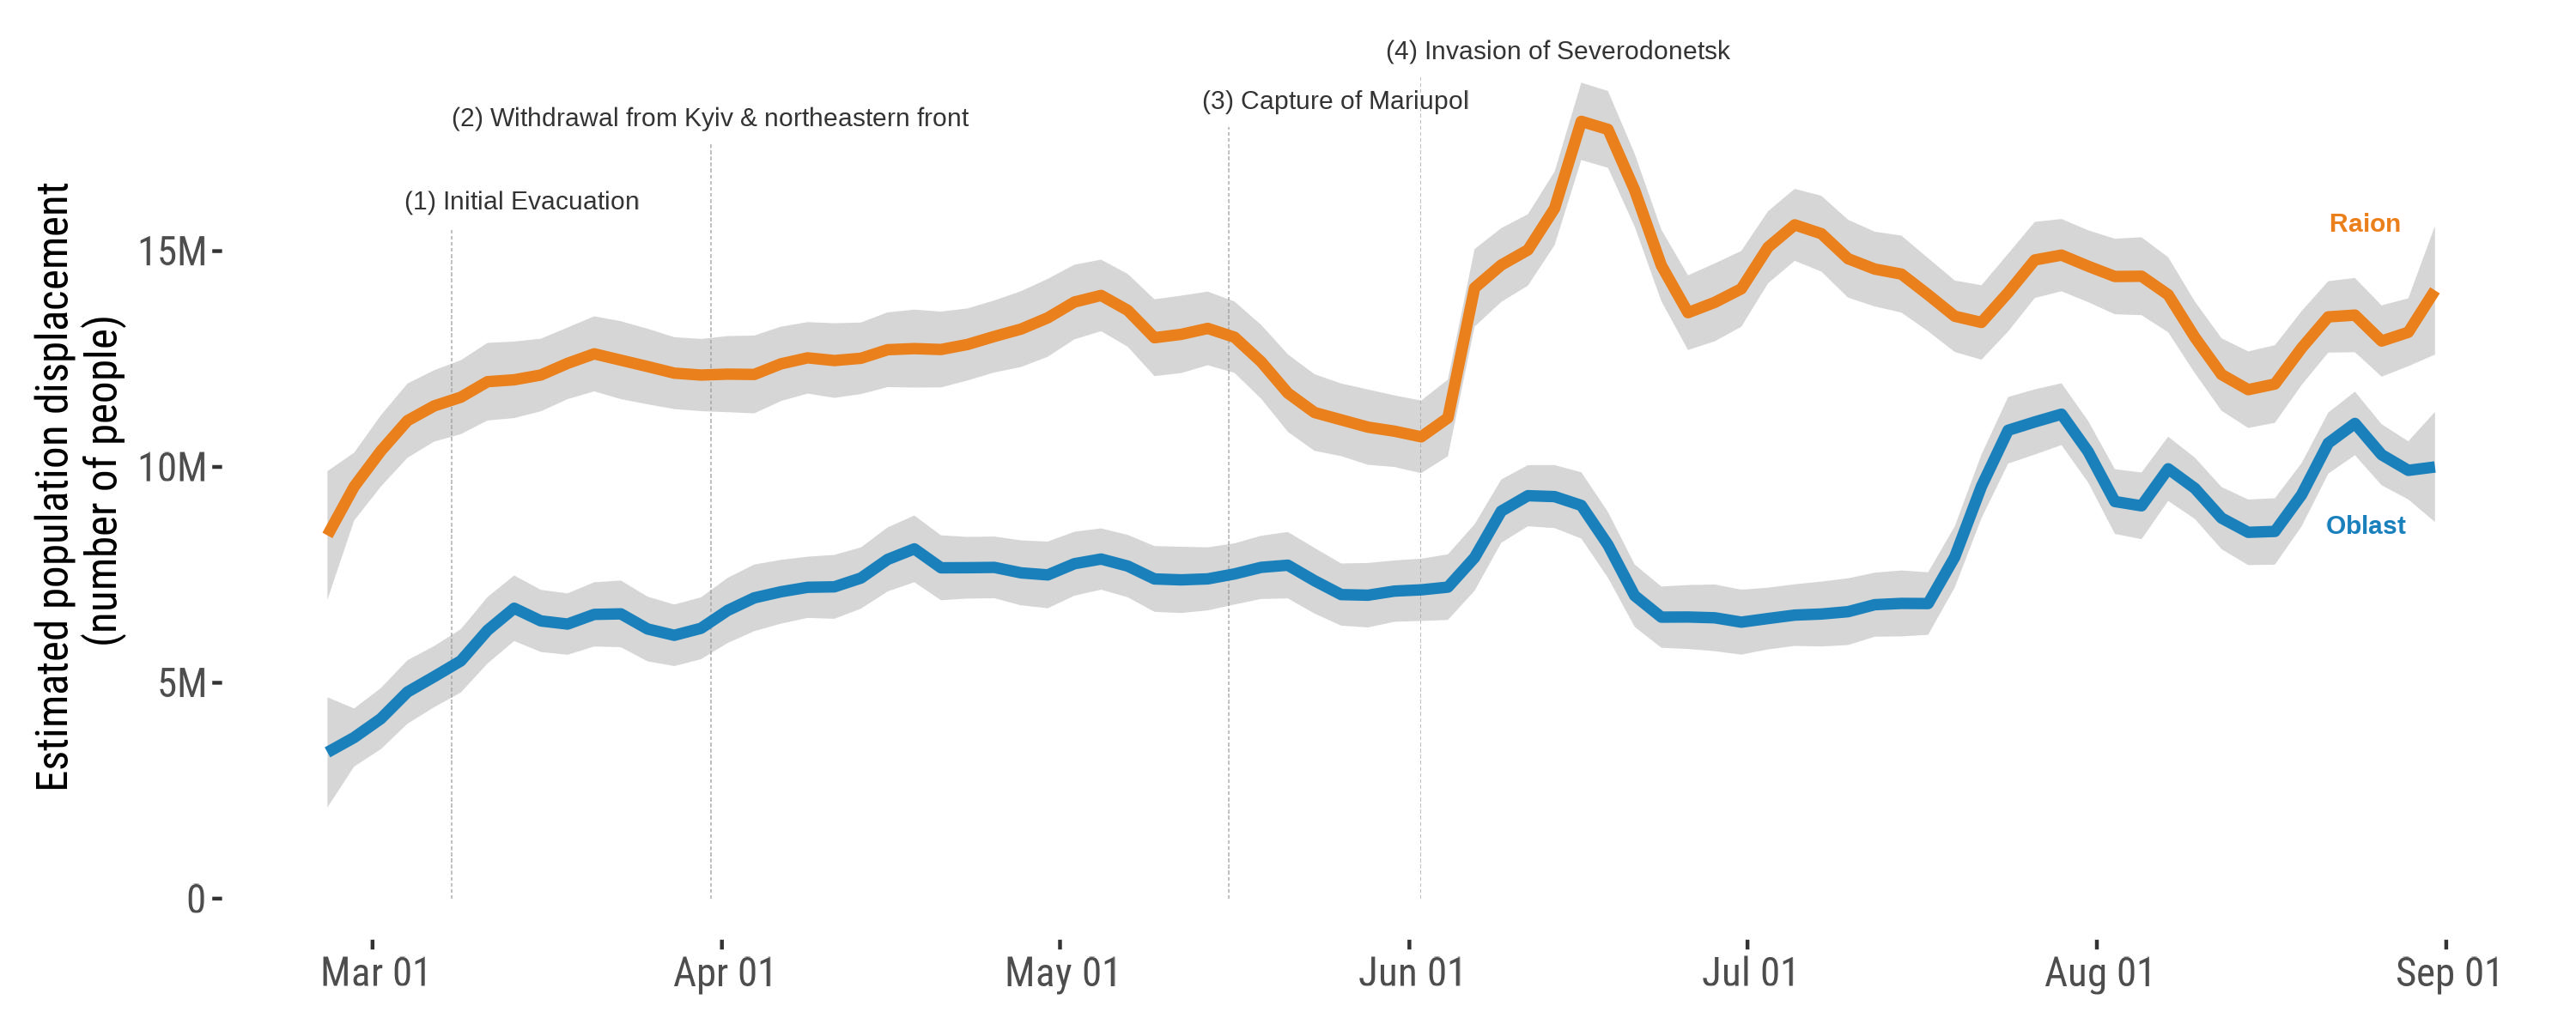
\includegraphics[keepaspectratio]{../outputs/2_1/fig1.jpg}}

\end{minipage}%

\caption{\label{fig-popdisplacement}\textbf{Estimated daily number of
displaced population. February to August 2022.} The number of displaced
people is estimated as the difference between the population in a region
for a given day after the start of the war and the population before the
war in 2020 - see Methods Section. Local polynomial regression modelling
was used to build 95\% confidence intervals.}

\end{figure}%

Our contribution is to generate geographically granular estimates of
internal displacement at the raion level leveraging the high spatial
precision of GPS data. As anticipated, the levels of raion-level
displacement consistently exceeds those of oblast-level displament as
they reflect movements that cannot be captured at higher levels of
spatial aggregation: raions within the same oblast's boundaries
capturing the fact that most displacement tends to occur over short
distances. Our raion-level estimates indicate a rise and peak of over 17
million displaced people in mid June 2022 following the start of the
Russian invasion of Severodonetsk. Around 90\% of the buildings and
infrastructure is estimated to have been destroyed or damaged after the
capture of Severodonetsk (Dlugy 2022). From mid July, our estimates
indicate a rise in population displacement at the oblast level, but such
increase is not reflected at the raion level, indicating that the most
displacement that took place during this time tended to occur over long
distances involving a cross of oblast boundaries (see Fig.1 in the
Supplementary Material (SM) displaying distance distributions).

Our findings are consistent with existing estimates. We compare our
oblast-level displacement estimates with existing estimates derived from
an United Nations - International Organization for Migration (IOM)
survey (IOM 2022b) and Facebook data (Leasure et al. 2023) (see Methods
Section, Table 1 and Figures 2-4 in SM). The shape of the temporal
evolution of population displacement is remarkably consistent. Though,
we identify some discrepancies. Our estimates tend to be higher than
those produced by Leasure et al.~by approximately 250 thousand people
across the time series. The difference can be explained by Leasure et
al.'s estimates are affected by power outages in the Donetsk and Luhansk
regions resulting in zero or small numbers for various dates (Rowe,
Neville, and González-Leonardo 2022; Leasure et al. 2023) (see Figure 3
in SM). Similarly, our oblast-level estimates are noticable greater than
the IOM figures in June and August. We assume that this is because our
estimates include data from Crimea, and there was significant movement
from and to Crimea to Russian-occupied Ukrainian territory and Russia
during these months (Walker 2024). This is as Russia started a
``volunteer mobilisation'' and deployed new troops and logistics to
support an a frontline extending from Zaporizhzhia to Kherson, along the
Dnieper River (Walker 2024). If we exclude Crimea, our estimates are
much closer to IOM and Leasure et al.'s estimates (see Table 1 in SM).

\subsection{Identifying the main origins and
destinations}\label{sec-odm}

We then examine the net balance of internal population displacements
resulting inflows minus outflows, to identify the main areas losing and
gaining population through these displacements. As expected,
Figure~\ref{fig-heatmaps}a reveals that Kiev City was the main area
losing population at the start of the war between late February and
early May before recording large positive net balances of over 2 million
people. These gains seem to echo large-scale return population movements
as Russian troops withdrew from the outskirts of Kiev City and focused
on the eastern and southern regions of Ukraine, particularly Donetsk,
Kharkiv, Crimea and Luhansk (Figure~\ref{fig-heatmaps}b). Reflecting the
geographic concentration of military ground forces, these frontline
eastern and southern regions registered a consistent pattern of
population losses between March and August. Population losses are
particularly prominent in Donetsk where the estimated losses exceeded 2
million people in late July and early August 2022. To a lesser extent,
Odessa also displays a negative albeit moderate balance of population
displacements during the early months of the invasion as Russia had a
naval blockade on Ukrainian ports.

\begin{figure}

\begin{minipage}{\linewidth}

\includegraphics[width=\linewidth,height=0.8\textheight,keepaspectratio]{../outputs/2_2/fig2-two-partsa.pdf}

\end{minipage}%

\caption{\label{fig-heatmaps}\textbf{Net migration count by oblast and
raions, February to August 2022.} \textbf{a.} Weekly median net
migration by oblast. \textbf{b.} Monthly median net migration across
raions. \textbf{c.} Changes in the share of estimated population across
the urban-rural hierarchy.}

\end{figure}%

\begin{figure}

\begin{minipage}{\linewidth}

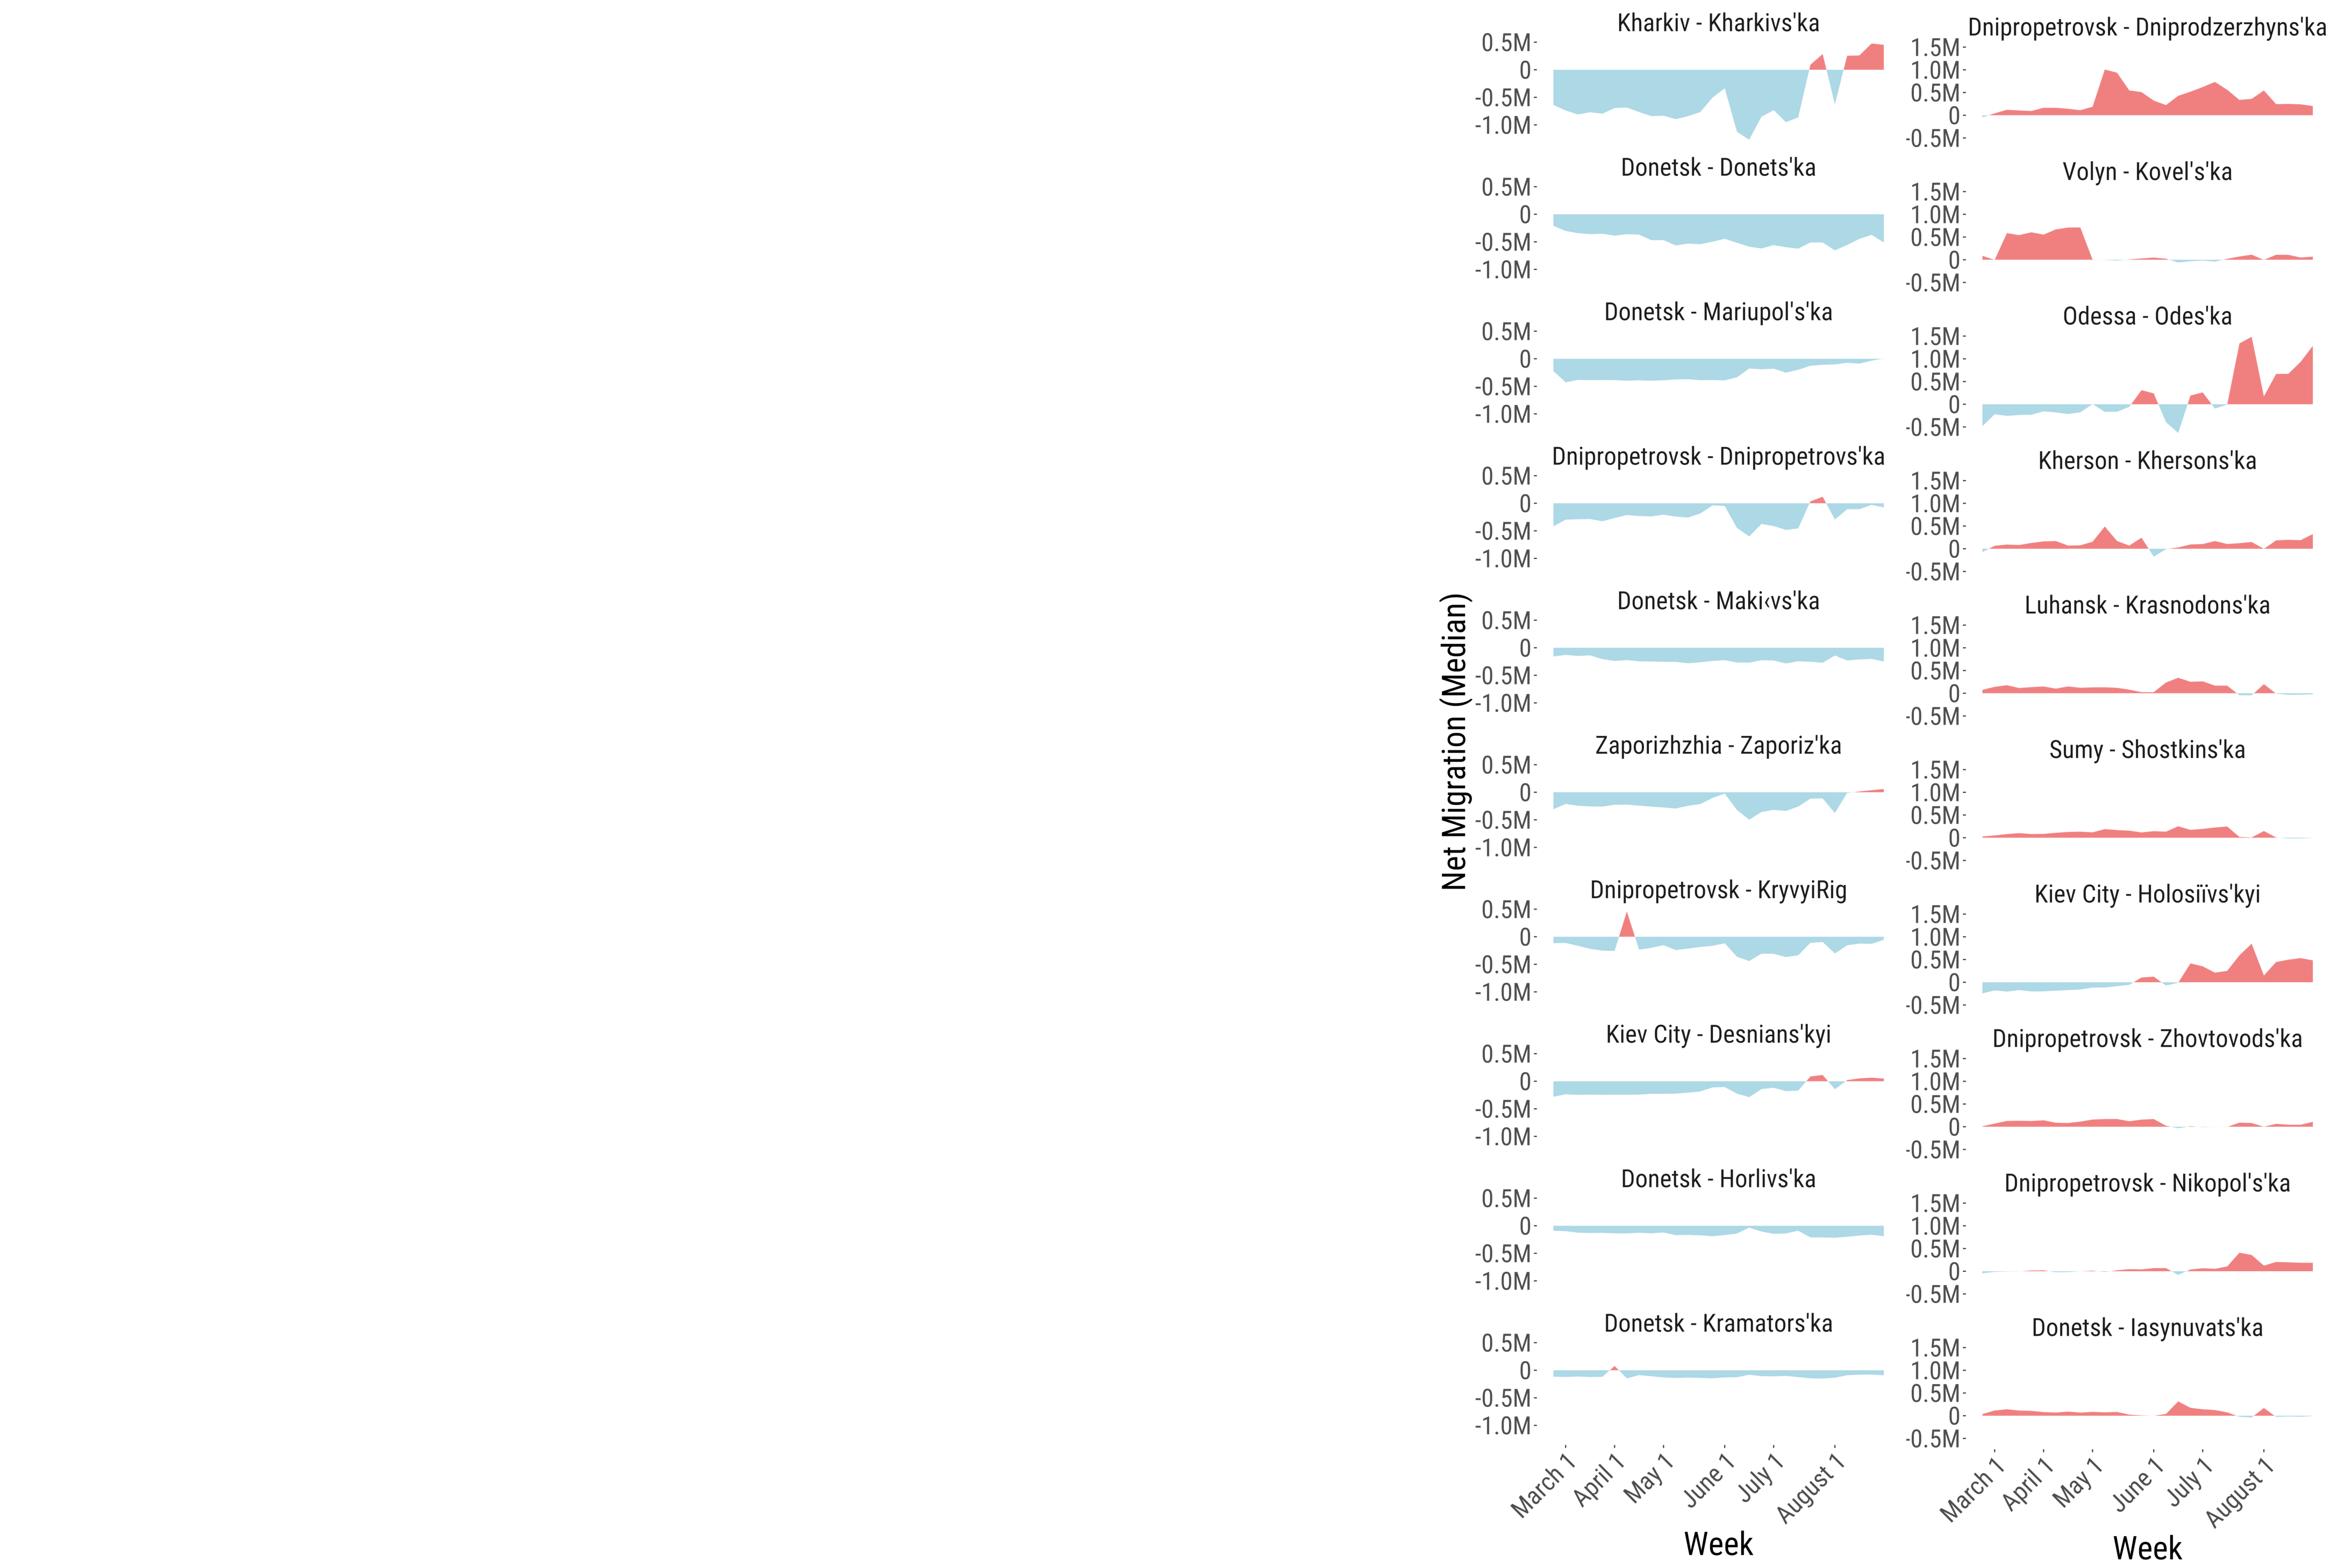
\includegraphics[width=\linewidth,height=1\textheight,keepaspectratio]{../outputs/2_2/fig2-two-partsb.pdf}

\end{minipage}%

\caption{\label{fig-heatmaps2}\textbf{Top ten raions with the largest
cumulative net negative (in blue) and positive (in red) migration
balance organised from the largest to the smallest, February to August
2022.}}

\end{figure}%

At the same time, Figure~\ref{fig-heatmaps}a reveals that western,
central and central-south areas tended to gain population during the
early months of the invasion between February and June 2022. These areas
include oblasts close to the border with Poland, Slovakia, Hungary,
Romania and Moldova, such as Ivano-Frankivs'k, Vinnytsya, Volyn and
Zakarpattia probably serving as transit centres for international
crossings and humanitarian assistance. Kirovohrad also shows
considerable positive population balances over the early months of the
war, most likely receiving population from frontline areas in eastern
parts of Ukraine. Figure~\ref{fig-heatmaps}a shows that most of these
areas have tended to experience population losses as Kiev City and
Odessa record positive population balances from late July.

These aggregate patterns of population displacement conceal the local
concentration of net population losses and gains across raions.
Figure~\ref{fig-heatmaps2} reports the net balance of population
displacements over time for the ten raions with the largest cumulative
losses and gains between February and August 2022. It reveals that
Kharkiv remained the raion with the largest cumulative loss of
population since the start of the war at least until August 2022, but it
reported positive balances as Ukrainian forces launched a
counteroffensive and liberated major settlements in the Kharkiv oblast
in late July and August 2022. The oblast of Donest'k seems to congregate
the raions with the greatest population losses, reflecting the
concentration of frontline activity in raions, such as Donets'ka,
Mariupol's'ka and Makivs'ka.

On the other hand, Figure~\ref{fig-heatmaps2} reveals that raions within
the oblasts of Dnipropetrovsk, Kiev City and Donetsk recorded the
largest cumulative net migration gains at times when these oblasts
recorded moderate overall net migration losses
(Figure~\ref{fig-heatmaps}a). The raions of Dniprodzerzhyns'ka,
Zhotovods'ka and Nikopol's'ka all registered large cumulative population
gains through net migration from February to August 2022 despite
systematic moderate overall negative migration balances in the oblast of
Dnipropetrovs'k. Similarly, the raion of lasynuvats'ka in Donestk
recorded a large cumulative net migration gain despite this being the
oblast with the largest negative migration balances. These results
suggest that people tended to move locally to neighbouring areas, or
were unable to afford moving to more distant locations in western
Ukraine (see Figure 1 in SM).

Additionally, mapping the patterns of net migration
(Figure~\ref{fig-heatmaps}b and Figure~\ref{fig-heatmaps}c) reveals the
increasing prevalence of population loss through net migration in
Ukraine, particularly in less populated areas. In early weeks of the
invasion in February, negative net migration balances concentrated in
urban centres, especially Kiev and Khakiv. As the conflict evolved, net
migration losses seem to have expanded to most of the country
prominently reducing the relative national share of population in very
low density and low density rural areas (Figure~\ref{fig-heatmaps}c).
These reductions in sparsely populous areas appear to have been mirrored
by a growing national share of population in urban centres, with Kiev
and Odessa acting as the major centres of population attraction in
August (Figure~\ref{fig-heatmaps}c).

\subsection{Measuring the rate of return movements}\label{sec-return}

Understanding the scale and pace of return movement to residential areas
in conflict zones after a period of displacement is also important to
shape and support humanitarian assistance, successful reintegration,
mental health and community rebuilding programmes (Galindo 2023).
Understanding return movements enables more efficient resource
allocation prioritising areas for infrastructure reconstruction and
service delivery (Galindo 2023). IOM estimated that 6 million people had
returned to their usual place of residence in Ukraine by August 23 2022
following a two-week period elsewhere in the country (UNHCR 2023). At
the time of writing, the most recent IOM estimate puts this figure at
4.7 million returnees in April 11 2024, 14.2 per cent of whom returned
from abroad (IOM 2024). These estimates are derived from a survey of 20
thousand people, with follow-ups to 1,638 individuals identified as
returnees (IOM 2024). The proportion of returnees for each oblast is
computed and multiplied by the total population in Ukraine to derive
return estimates. Returnees are identified as those respondents who
spent a two-week period away from their place of residence.

\begin{figure}

\begin{minipage}{\linewidth}

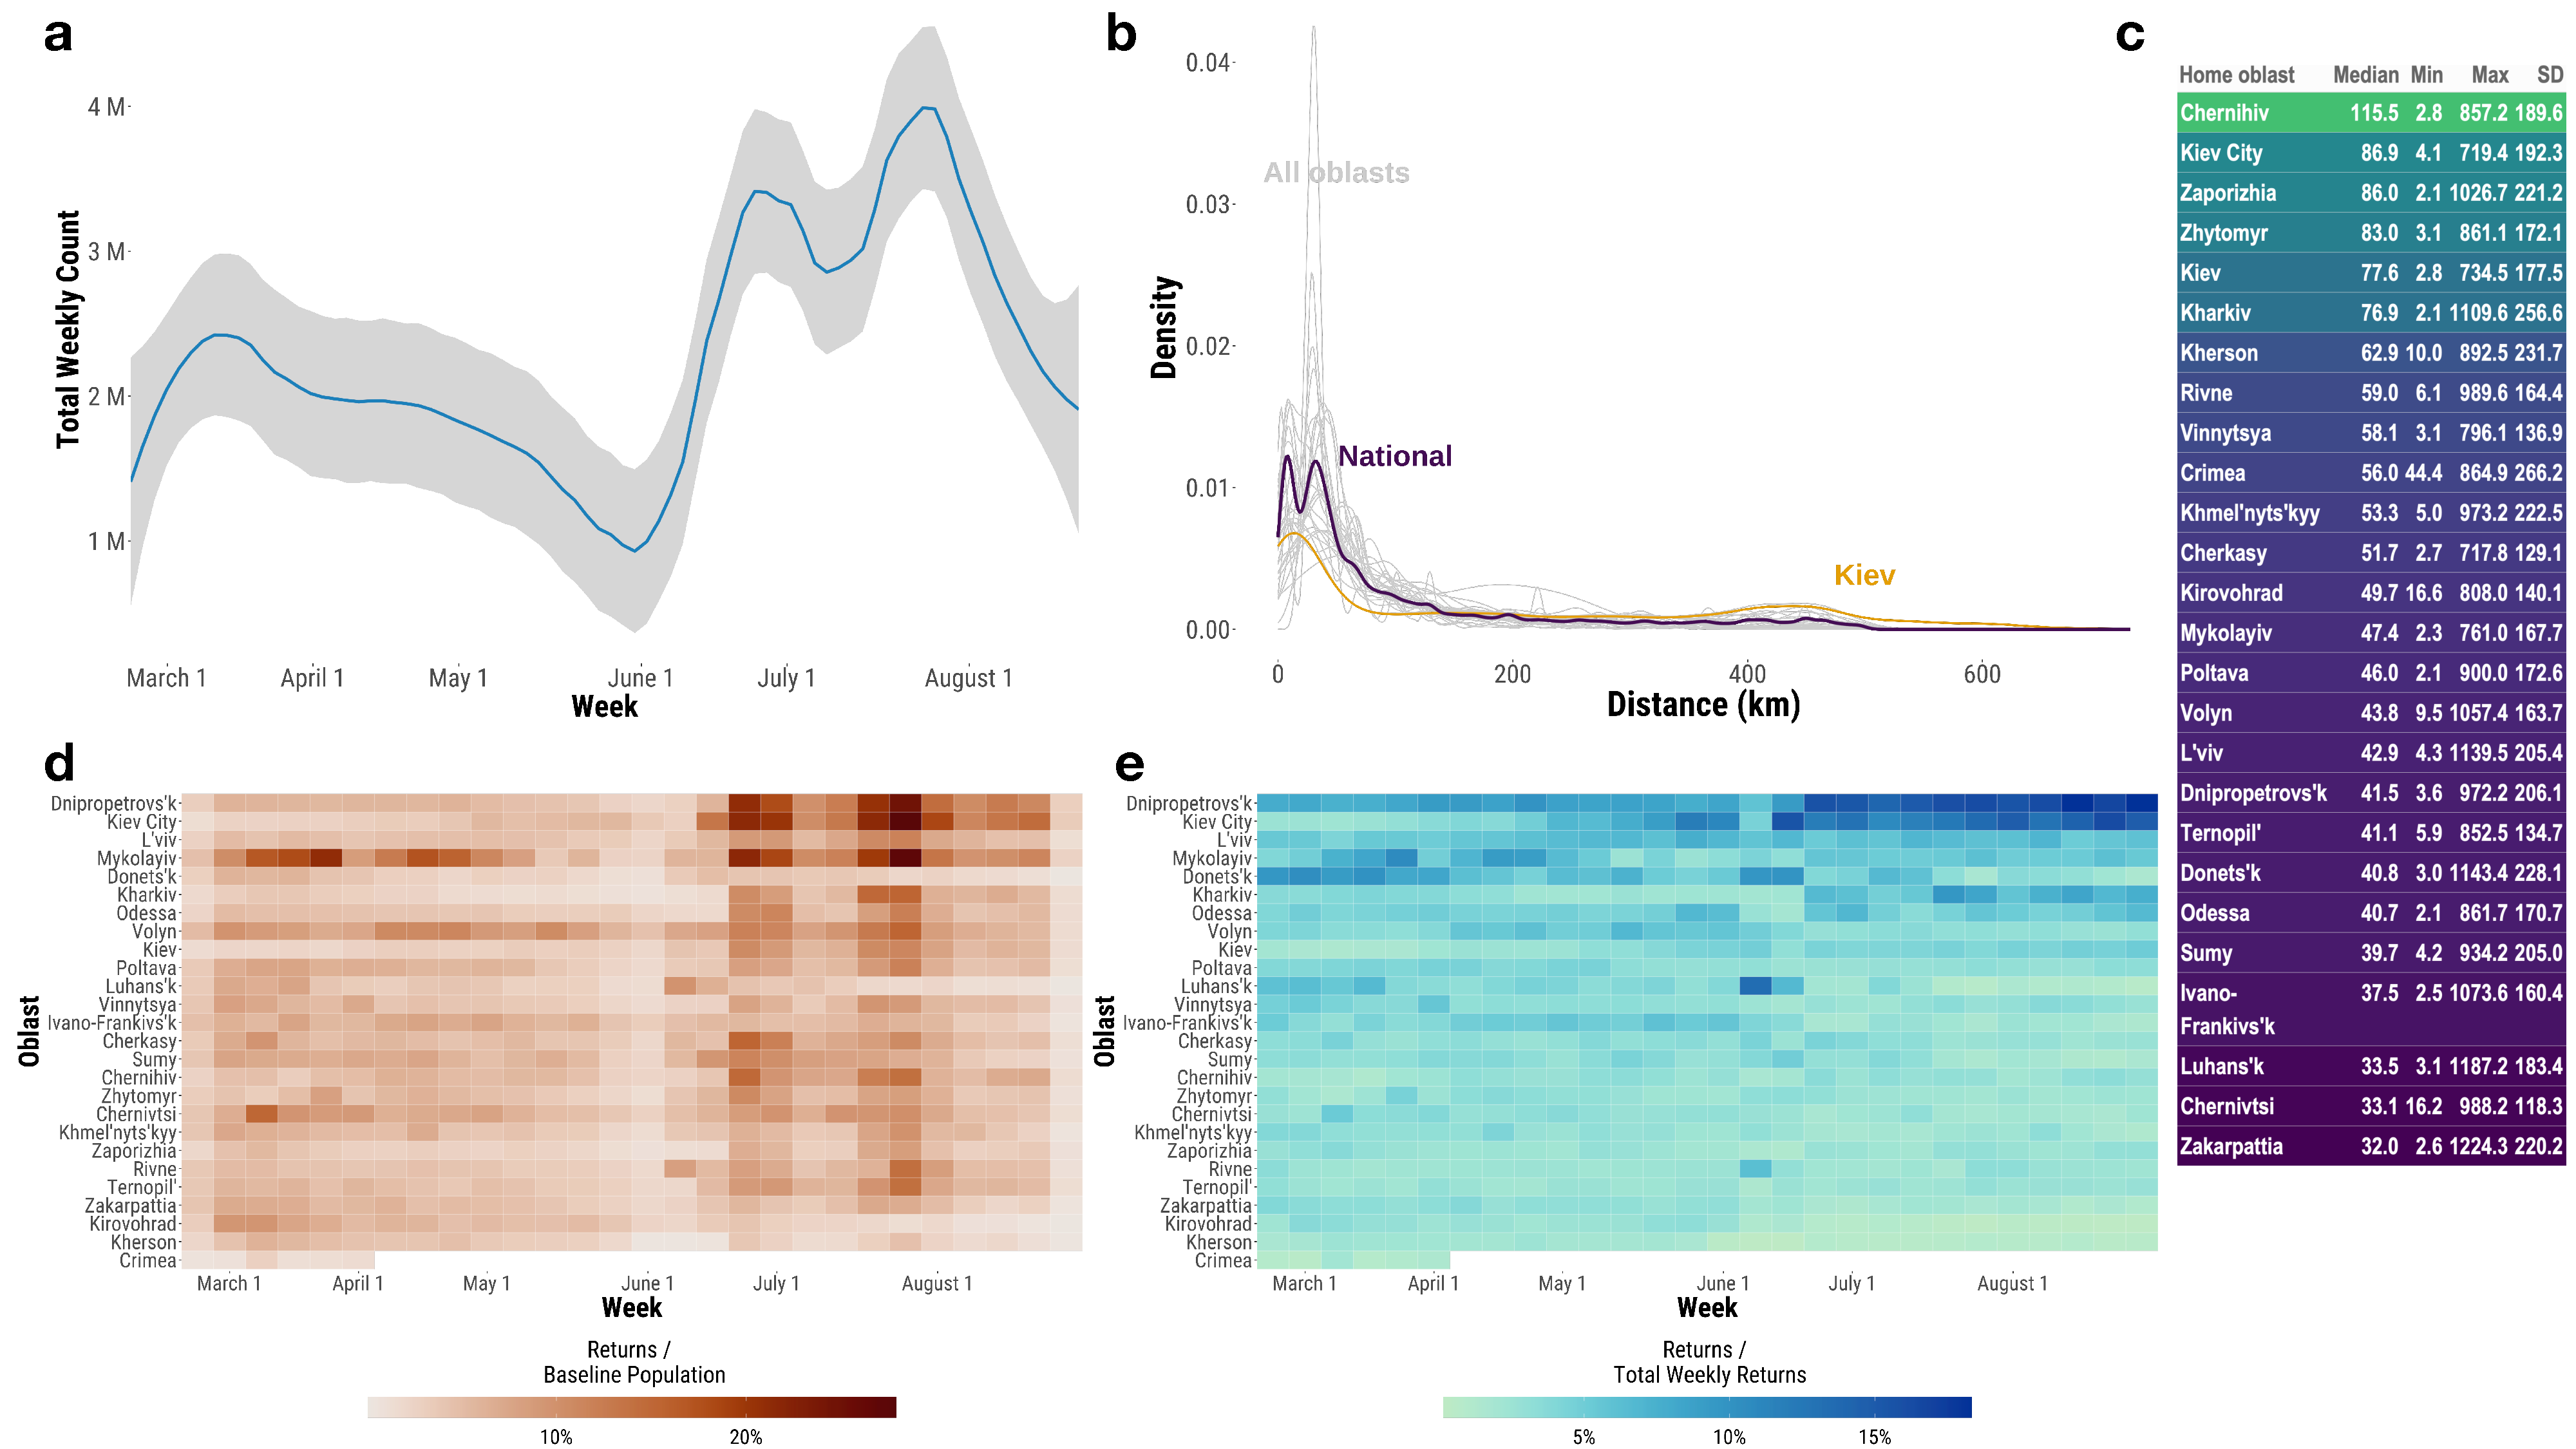
\includegraphics[width=\linewidth,height=0.6\textheight,keepaspectratio]{../outputs/2_3/dougs_returns/fig3.pdf}

\end{minipage}%

\caption{\label{fig-returns}\textbf{Return movements, February to August
2022.} \textbf{a.} Weekly total number of returns. Local polynomial
regression modelling was used to build 95\% confidence intervals.
\textbf{b.} Distribution of distance truncated to display return
movements below 700km. \textbf{c.} Median, minimum (min), maximum (max)
and standard deviation (SD) distance in km, oblast. \textbf{d.} Per cent
of returns over the total baseline population for individual oblasts
before the start of the war. \textbf{e.} Per cent of returns over the
total number of returns for individual oblasts.}

\end{figure}%

Using our methodology (see Methods Section), we generate estimates and
expand this evidence providing information on the spatial patterns,
distance and pace of return movements (Figure~\ref{fig-returns}a-e). Our
estimates indicate that just over 2 million people had returned to their
place of residence before February 24 during the week commencing August
22, 2022 (Figure~\ref{fig-returns}a). Our estimates also showed
considerable fluctuations over time, reflecting that some of
displacements and returns may be temporary. Some people may return to
their home location after spending a short period of time elsewhere.
Some may return to check on close relatives and friends, examine local
livability and recover belongings, and then leave. Our estimates
indicate that the average number of weeks associated with return moves
to a home location is nine weeks (see Figure 6 in SM). The fluctuations
observed in our estimates also reflect the fact that we are unable to
follow the same mobile phone devices for the entire period of analysis.
We observe some individual returns to the same location, but are unable
to identify their location in subsequent periods. Crimea is a good
example as we could only identify returns until the first week of April
but not thereafter (Figure~\ref{fig-returns}d-e).

Figure~\ref{fig-returns}d-e reveal a differentiated rate of return
movements across oblasts. Dnipropetrovs'k and Kiev City display higher
proportions of return movements relative to their populations before the
start of the armed conflict, and to the total weekly number of returns
across Ukraine. L'viv and Mykolaiv record high rates of return movement
likely reflecting their role as transit points, food, temporary shelter
and accommodation centres for refugees, IDP and troops
(González-Leonardo et al. 2024). Kherson and Crimea register the lowest
number of returns. As indicated above, no returns were recorded for
Crimea after April 2022, and Kherson remained under Russian occupation
during our period of analysis.

Return movements tend to occur over relatively short distances
(Figure~\ref{fig-returns}b-c). The median distance of return moves
between oblasts is less than 100km suggesting that most IDP tend to stay
relatively close to their home location. Global estimates indicate that
a median distance of less than 100km for internal migration moves is
common (Stillwell et al. 2016). However, a wide variation exists as a
function of the place of residence. IDP seem to be willing to travel
longer distances to return Chernivhiv, Kiev City and Zaporizhia than to
Luhans'k, Chernivtsi and Zakarpattia. Chernivhiv and Kiev City recorded
large flows of return movements as Russian troops withdrew from northern
areas of Ukraine and intensifies their war effort on eastern and
southern parts of the country.

\section{Discussion}\label{discussion}

We developed an approach to produce highly granular temporal and spatial
population-level estimates to monitor the extent and geographic patterns
of population displacement in disaster areas drawing on a large dataset
of GPS location data from mobile phone devices. Highly granular data of
internal displacement is essential for real-time monitoring to support
disaster relief and management efforts. Traditional data streams are
limited in their ability to generate such granular information in real
time during times of conflict or natural disasters. Focusing on the
unfolding invasion of Ukraine, we estimated that an increasing number of
people were displaced from their place of residence, with an average of
11 million people being displaced from their Oblast of residence and
over 15 million at the raion level at the start of the Battle of Bakhmut
in early August 2022.

We generated population-level estimates using smartphone location data.
However, validating the resulting spatially granular estimates remains a
significant challenge. Normally no comparable estimates exist to
evaluate the extent to which they capture the facts on the ground. That
is the reason why they are produced in the first place. Future efforts
could thus concentrate on making available a repository of high quality
datasets, such as data from comprehensive population registry or
administrative sources that can be used to assess the accuracy of
population-level estimates derived from digital trace data, such as
smartphone data.

We are unable to characterise the population being displaced or their
underpinning reasons using smartphone data. As most digitally generated
data, these data only offer location-time information. They do not
provide socio-demographic information about users or their motivations.
As such, we cannot identify the socio-demographic profile of displaced
individuals or why they move; yet, this information is critical to
deliver an appropriate humanitarian response. To tackle this, future
work could assess the integration of area-level data of the resident
population with highly granular displacement estimates derived from GPS
location data to more accurately capture the socio-demographic profile
of displaced communities, and surveys collecting information on why
people move.

We cannot discern between permanent and semi-permanent returns. We can
infer returns if individuals are back to their place of residence
recorded before the start of the war. However, the records of individual
mobile devices offer a rather irregular longitudinal sequence of
locations to confidently determine the time they remained in their place
of residence observed before the start of the war. Future work could
seek to secure a data over a longer time frame which may provide a
larger set of locations over time to distinguish between permanent and
semi-permanent returns.

Future work will need to address a key challenge; that is, accessibility
to mobile phone data. These data are routinely and globally collected,
but their access remains limited. Privacy and anonymity concerns and
regulation constrain their wide availability. While efforts have been
made to democratise data access and sharing via data services and data
for social good initiatives, such as Meta's Data for Good (Rowe et al.
2024), accessibility to mobile phone data is often ad-hoc arrangement
and for specific actors (Rowe and González-Leonardo 2024). Such
arrangements create issues of data availability and equity, which may be
particularly prominent in conflict-affected or low-resource settings and
may impact the generalisability and scalability of our proposed
approach. At the same time, we believe that tangible applications of
mobile phone data, such as our analysis, illustrating their practical
usefulness offer an incentive for national and intergovernmental
institutions, such as the United Nations and European Commission, to
promote the creation of data sharing partnerships with data holders.
These agencies have a prime position to create the digital
infrastructure to ensure equal and secure access to nontraditional data
streams, such as mobile phone data for the social good.

Despite these limitations, we contributed a novel methodology to unleash
the use of high-frequency mobile phone data to produce population-level
estimates of internal displacement. It recognises that mobile phone
datasets only provide representation for a selected group of the
population and moves beyond only capturing rough signals to provide
actual population counts. We provided evidence indicating that urban
centres were the predominant locations of population displacement during
the early months of the invasion, with Kiev as the primary origin
reporting net migration losses of approximately 2 million. As the
conflict progressed in 2022, we showed widespread population losses
through internal displacements. Proportionally the share of population
in low density rural areas has reduced mirroring a larger share of
population in urban centres. We showed a systematic increase in the
number of return movements to Kiev City following the withdrawal of
Russian forces from the northern and western front of the city, with
frontline areas continuing to lose population throughout the conflict.

Our work complements existing efforts to generate rapid response
estimates. To estimate population displacement in Ukraine, the IOM
designed a random digit dial telephone survey to produce a nationally
representative sample of 2,000 individuals during each monthly round
(IOM 2022a). However, this method of data collection is unable to: (i)
generate population level estimates to make inferences of the geographic
patterns of population displacement; (ii) offer temporally granular
frequency estimates (e.g.~daily or weekly) to monitor rapidly changing
population dynamics; or, (iii) produce high spatial resolution counts to
identify areas of humanitarian assistance with high precision (Leasure
et al. 2023). Prior work has explored the use of location data from
mobile and social media data to address these issues (Graells-Garrido et
al. 2021; González-Leonardo et al. 2024). Yet these efforts have been
restricted to provide rough signals of population movements indicating
the direction of trends, spatial patterns and changes of population
flows over time (Rowe 2023).

By using pre-conflict population data, we contributed to an approach
that is capable to adjust location data from mobile phone users, moving
away from offering rough signals, to provide estimates of the extent of
population movements. Our approach also has the capacity to provide
real-time monitoring of population displacement at highly temporally and
spatially adaptable resolutions. Our approach can thus complement
existing data resources aiming to provide a national-scale estimate of
population movement. In fact, our estimates aggregated at the national
level were consistent with those derived from the IOM telephone surveys
(IOM 2022a) and social media data (Leasure et al. 2023). The
triangulation of estimates across these sources helps build confidence
in the official UN estimates, but also on estimates leveraging
innovative data.

\section{Methods}\label{methods}

\subsection{Data sources}\label{sec-data-sources}

\textbf{Global Positioning System (GPS) location data.} The primary
source consists of GPS location data from 25 million unique mobile phone
devices located within Ukraine. The data include hourly GPS locations
(longitude and latitude) in Ukraine, their accuracy and time stamps from
January 1st 2022 to August 31st 2022. Data from digital mobile phone
applications are known to contain biases as they typically represent the
behaviour of a segment of the population (Rowe 2023). To mitigate any
potential biases from the use of information from a single source, we
use data collected from a range of mobile applications comprising a
variety of users and purposes. Ethical considerations prevent us from
identifying these applications. The data were obtained from a data
vendor.

We process the data to identify unique devices with locations recorded
before (January 1 to February 24, 2022) and after (February 25 to August
31, 2022) the start of the escalation of the Ukraine-Russia conflict. We
identify 17 million devices (approximately 70\% of the total) with
locations before the February 24, and 13 million (approximately 55\% of
the total) with recorded locations after the escalation of the conflict.
We identify 6 million devices with recorded location information for
both before and after the full-scale invasion on February 24, 2022.

To further analyse the data, we apply three main procedures. First, we
apply a point-to-polygon spatial join to assign latitude and longitude
coordinates to administrative boundaries (raions and oblasts) and
settlement area type as defined by the Global Human Settlement Layer
(GHSL) - see description below in Geographic data. Second, we convert
UNIX time stamps into local Ukrainian date and time. Third, we infer
individual home locations for each mobile phone device. For this, we
follow the UN guidelines on official statistics using mobile phone data
(Magpantay et al. 2022), and define home location as the place where a
mobile phone is recorded most of the time during night (i.e.~between 7pm
and 5.59am). We used observations with at least 3 observations during
these hours. We calculated the number of days a user's mobile phone
device was detected in the same location during these nighttime hours.
We consider the location where a user's mobile phone device was recorded
for more than 50\% of their time as their place of usual residence
(Magpantay et al. 2022).

To provide a sense of the representativeness of the mobile phone data
used and our resulting population-level estimates, we performed
correlation analysis at the oblast and raion levels
(Figure~\ref{fig-data-coverage}a-b). We analysed the correlation (1)
between the size of our pre-war baseline population and number of unique
mobile phone devices; and, (2) between the size of the pre-war baseline
population and our proposed population-level estimates. We included the
mobile phone penetration rate representing the size of each dot on the
scatter plots, to provide a sense of population coverage in each area.
Figure~\ref{fig-data-coverage}c reveals that our mobile phone data
provides good population coverage across the country, with 91\% of
raions displaying a penetration rate of over 30\%. Coverage tends to be
greater around the regions of Kiev and Chernivtsi, and lower in Crimea
and the Chornobyl Exclusion Zone. Correlation coefficients over 0.76
indicate a high degree of representativeness of our ``raw'' unique
mobile devices at both the oblast and raion levels. The high degree of
correspondence indicates that our mobile phone data provide a good
representation of the pre-war population across sparsely populated areas
(such as Verkhovynskyi, Novhorod-Siverskyi and Svativskyi) and large
urban centres (such as Kyiv, Kharkivskyi and Donetskyi) along the
rural-urban hierarchy. Correlation coefficients of .9 and 1 reflect an
even high degree of representativeness of our proposed population-level
estimates and pre-war population data. For oblasts, the correlation is
slightly lower because we used census population data for our
correlation analysis. For raions, we used WorldPop data as explained
below because census population data were not available.

\begin{figure}

\begin{minipage}{\linewidth}

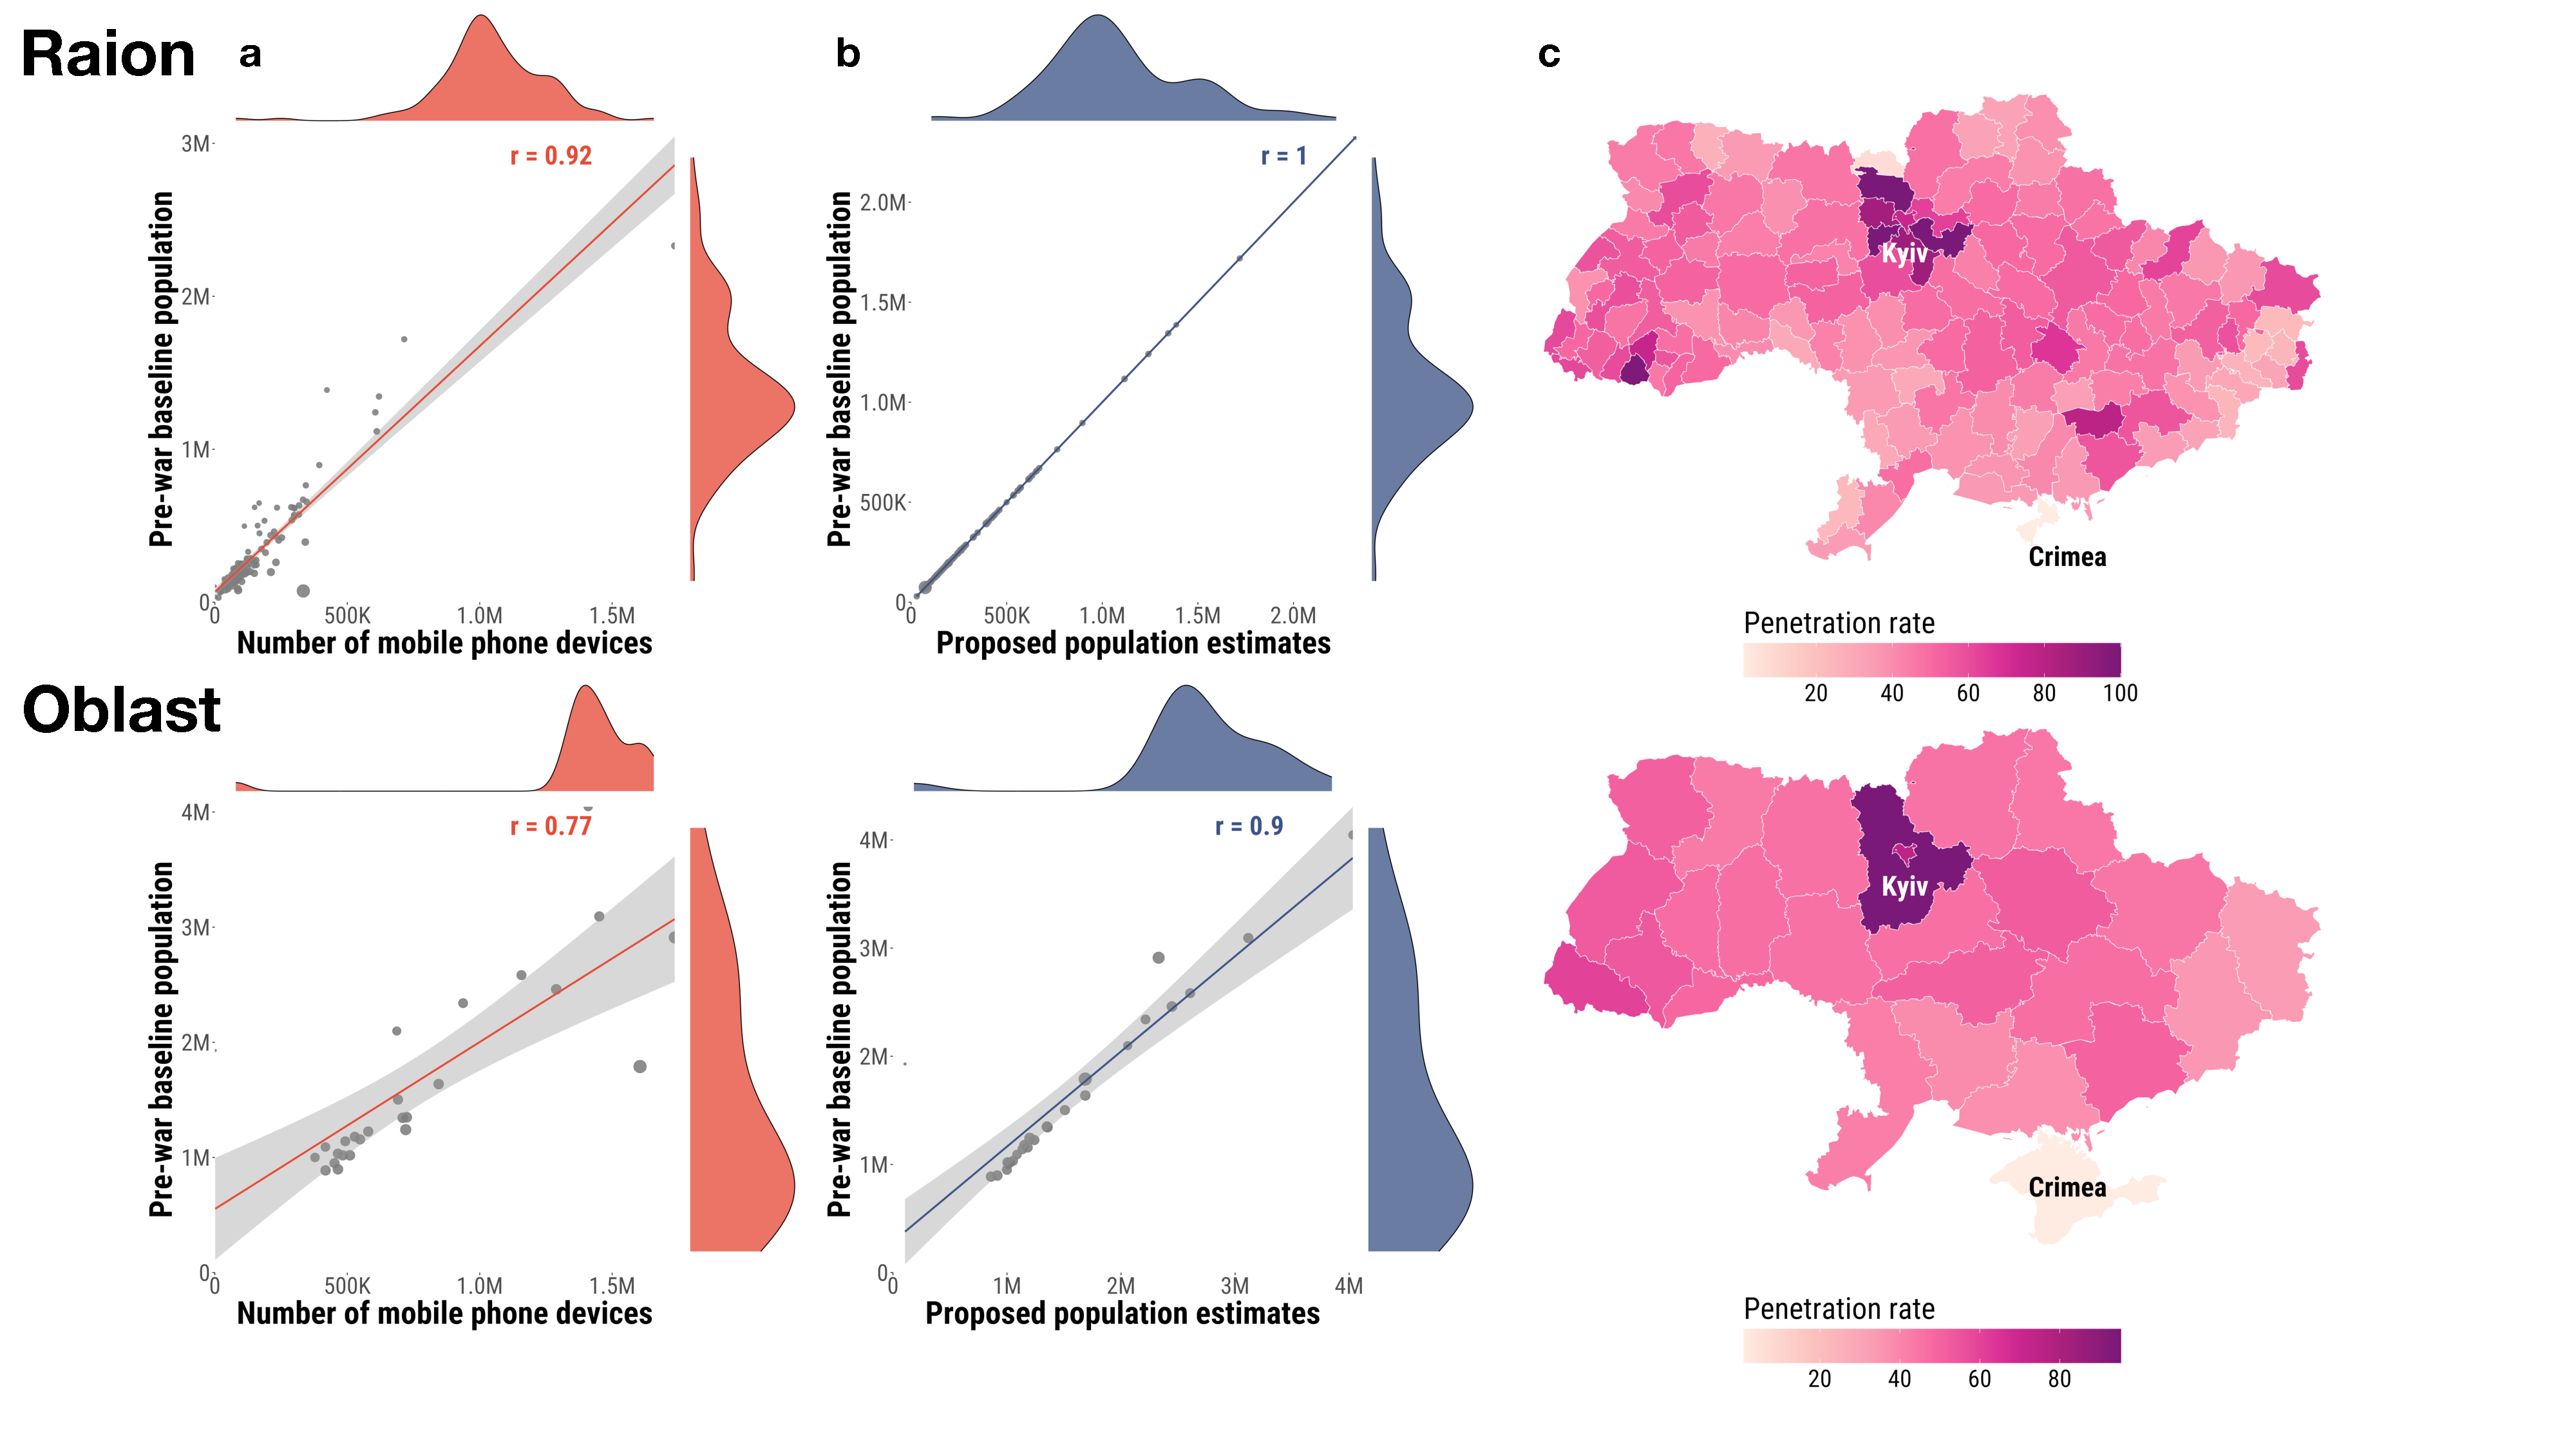
\includegraphics[width=\linewidth,height=0.8\textheight,keepaspectratio]{../outputs/2_4/mp-data-coverage.pdf}

\end{minipage}%

\caption{\label{fig-data-coverage}\textbf{Correlation between pre-war
baseline population estimates and mobile phone data coverage at raion
and oblast levels.} \textbf{a.} Correlation between pre-war baseline
population, and number of unique mobile phone devices in February 2022
before the start of the war. \textbf{b.} Correlation between pre-war
baseline population, and our proposed pre-war population post adjustment
for estimates in February 2022 before the start of the war. \textbf{c.}
Penetration rate as the number of unique mobile phone devices over the
pre-war population. Spatially aggregated population counts from WorlPop
are used for the pre-war baseline population. Size of dots represent the
local penetration rate. Local polynomial regression modelling was used
to build 95\% confidence intervals.}

\end{figure}%

\textbf{Baseline population data.} We use \(100m^{2}\) gridded
population data to establish the baseline population before the conflict
in Ukraine in 2020 (WorldPop n.d.). We utilise unconstrained population
estimates from \href{https://www.worldpop.org/}{worldpop.org}. These
were the most up-to-date population estimates available for our
analysis. We spatially aggregate the WorldPop population counts to
create baseline population datasets at the raion and oblast levels.
These population estimates are then used to derive population-level
estimates of internal displacement, as described below.

\textbf{Refugee data.} We use United Nations High Commissioner for
Refugees (UNHCR) daily counts of people entering and leaving Ukraine
(UNHCR 2024). We accessed these data from an archived version of the
UNHCR website available via \href{https://web.archive.org/}{The Internet
Archive}. These data included daily cross-border movement records from
the start of the full-scale invasion in Ukraine until August 16 2022. We
calculate a cumulative net count by subtracting the number of people
entering Ukraine from those leaving the country. We use this count to
more accurately estimate the number of internally displaced people in
Ukraine by discounting the number of people who moved overseas from the
baseline population.

\textbf{Geographic data.} We use data from two sources. First, we use
geopackages containing the administrative boundaries of Ukraine,
particularly raions and oblasts. We draw on geospatial vector data from
the United Nations Office for the Coordination of Humanitarian Affairs
(OCHA) \href{https://data.humdata.org/dataset?}{Humanitarian Data
Exchange (HDX) data portal} and \href{https://gadm.org/}{Global
Administrative Areas} (GADM) (GADM 2022). We first spatially join our
GPS mobility data with GADM raion and oblast boundaries. GADM boundaries
contain 629 raions and 26 oblasts. We then aggregate these raions based
on HDX raion boundaries which correspond to the offically recognised
administrative boundaries in Ukraine.

We also use the degree of urbanisation classification from the
\href{https://human-settlement.emergency.copernicus.eu/}{GHSL} to
determine the type of settlement areas of IDP, both origins and
destinations. We reclassify the seven original categories to identify
three types of areas: urban (dense urban cluster and urban centre),
suburban or peri-urban (suburban and semi-dense urban cluster), and
rural (very low density rural, low density rural and rural cluster)
(Florczyk et al. 2019).

\subsection{Computation of population-level displacement
estimates}\label{sec-methods2.2}

\textbf{Estimating Internal Displacement.} We obtain population-level
estimates of internal displacement by correcting population counts
derived from the identified home location based on our smartphone GPS
data, to make them representative of the overall population. That is, we
correct mobile phone-derived population estimates to account for
differences in the use of mobile phone technology across locations in
Ukraine and over time. To this end, we adapted a deterministic model
proposed by Leasure and colleagues (Leasure et al. 2023). Intuitively
the approach involves first establishing our baseline population; that
is the pre-war population of Ukraine. We use population data from
WorldPop for 2020. Second, we identify the baseline number of mobile
phone users in Ukraine before the start of the full-scale invasion by
aggregating the number of unique devices in each home location based on
our GPS mobile phone data. Third, these two sets of baseline estimates
are used to compute the baseline mobile phone penetration rate in each
location \(i\) before the start of the full-scale invasion (\(t=0\)).
Formally, this rate can be expressed as:

\begin{equation}\phantomsection\label{eq-equation1}{ \psi_{i,t=0} = \frac {S_{i,t=0}} {N_{i,t=0}}}\end{equation}

where: \(S\) is the baseline median daily active mobile phone users
between January 1, 2022 to February 24, 2022; \(N\) is the baseline
total population in 2020 obtained from WorldPop.

Next, we estimate the present population \(N\) in location \(i\) at a
given point in time \(t\) from our GPS mobile phone data adjusting for
rate of mobile phone penetration. We do this by dividing the current
median daily active mobile phone users \(S\) at location \(i\) and time
\(t\) over the baseline smartphone penetration rate \(\psi\) at location
\(i\), assuming constant penetration rate since before the conflict:

\begin{equation}\phantomsection\label{eq-equation2}{ N_{i,t} = \frac {S_{i,t}} {\psi_{i}} }\end{equation}

We introduce a scaling factor (\(\theta\)) to account for potential
changes in mobile phone penetration rate over time as people leave
Ukraine and the local population shrinks. For this, we use daily
population counts of refugees from UNHCR and compute the net balance of
people leaving Ukraine which is denoted as \(R\). We compute the scaling
factor at time \(t\) using:

\begin{equation}\phantomsection\label{eq-equation3}{ \theta_{t} = \frac{\sum_{i=1}^I N_{i,t=0} - R_{t}}{\sum_{i=1}^I N_{i,t}} }\end{equation}

We use this scaling factor to compute our adjusted present population
(\(\hat{N}\)) multiplying the present population \(N\) obtained from
Equation~\ref{eq-equation2} and \(\theta\):

\begin{equation}\phantomsection\label{eq-equation4}{ \hat{N}_{i,t} = \theta_{t} N_{i,t} }\end{equation}

Using these population estimates, we can estimate changes in local
population across Ukraine over time. We can do this by subtracting our
adjusted current population estimates from the baseline population:

\begin{equation}\phantomsection\label{eq-equation5}{ \Delta_{i,t} = \hat{N}_{i,t} - N_{i,t=0}}\end{equation}

where: \(\Delta_{i,t}\) is the difference in population in location
\(i\) at time \(t\). For this difference, negative scores indicate a
local population loss due to internal population displacement, relative
to the baseline pre-war population. Similarly, positive scores indicate
a local population gain due to internal population displacement.

\textbf{Validation.} We assess the accuracy of our estimates of
population displacement. We measure the strength of the correspondence
between our set of mobile phone-based estimates \emph{versus} the
survey-based estimates produced by the IOM (IOM 2022b), and the
Facebook-based estimates produced by Leasure and colleagues (Leasure et
al. 2023). We do not anticipate a perfect linear relationship as
differences exist in the data source and methodologies to produce the
estimates. However, we do expect a high degree of correlation indicating
a high degree of temporal correspondence between estimates. We compared
against published IOM estimates at the national and regional levels
during the most of our analysis, and also oblast-level estimates
published by Leasure and colleagues. Unfortunately more comparable
spatially granular estimates at the raion level were not available for
our period of analysis. Supplementary Table 1 and Figures 2-4 display a
set of Pearson correlation coefficients, scatter plots and temporal
relationships between these and our estimates. The results reveal a high
degree of geographic and temporal correspondence between our estimates
and those produced by IOM and Leasure and colleagues across the set of
metrics.

\subsection{Displacement metrics}\label{sec-metrics}

\textbf{Net balance of displacement.} To identify areas of high internal
population displacement, we analyse temporal changes in the net balance
of internal displacement. We compute the weekly average net balance of
internal displacements (\(NET\)) as the subtraction of the number of
people arriving (\(IN\)) minus the number of people leaving an area
(\(OUT\)). Positive scores indicate a net balance population gain due to
internal displacement, while negative scores denote a net balance
population loss. The net balance of internal displacement is computed
as:

\begin{equation}\phantomsection\label{eq-equation6}{ NET_{i,t} = {IN_{i,t}} - {OUT_{i,t}} }\end{equation}

\textbf{Population change across the urban-rural hierarchy.} We analyse
changes in population across the urban-rural hierarchy. We hypothesise
that dense urban areas have attracted a disproportionate number of
internally displaced people as they tend to serve as centres of
protective infrastructure and services for civilians. At the same time,
we expect decreases in population due to internal displacement in rural
areas. To determine the extent of population changes, we compute the
percentage change in population in individual areas, relative to the
baseline population (Equation~\ref{eq-equation7}). For this, we
spatially aggregated our internal displacement estimates at raion to
settlement areas based on the GHSL degree of urbanisation classification
described in Data Sources Section.

\begin{equation}\phantomsection\label{eq-equation7}{ percent_{i,t} = \frac {\hat{N}_{i,t}} {N_{i,t0}} * 100 }\end{equation}

\textbf{Estimating returns.} We estimate the number of people who
returned to their usual place of residence before the start of the
full-scale invasion after a move somewhere else in the country. We
produce estimates at the raion and oblast level. We implemented and
compared two different approaches to estimate the number of returnees.
These approaches are based on the methods used by: (1) the IOM (IOM
2024); and, (2) Leasure and team (Leasure et al. 2023).

Similar to the former, we defined returns as those individual devices
which are recorded away for a period of at least two weeks and
subsequently in the same area identified as home location before the
start of the full-scale invasion. For individual areas, we computed the
relative proportion of return movements dividing the number of returns
relative to the total number of devices in a given home location. These
proportions are then multiplied by the pre-war baseline population to
produce population-level estimates of returnees.

Similar to Leasure and team, we defined returns as those individual
devices which are recorded away for an average of nine weeks and
subsequently in the same area identified as home location before the
start of the full-scale invasion (see Figure 6 in SM). Following the
same rationale explained for deriving our population-level estimates of
population displacement above, we divided the count of returns by the
pre-war smartphone penetration rate for each area. Acknowledging that
pre- and post-war smartphone penetration rates might differ as people
leaving Ukraine, we adjusted our estimates with scaling factors that
accounted for refugees who had left the country using
Equation~\ref{eq-equation3} and Equation~\ref{eq-equation4}.

We compared both sets of estimates and considered that the second
approach provides more reasonable estimates (see Figure 5 in SM). It
produces population-level return estimates displaying an increasing
trend, within the range of 1 million in February 2022 and 4 million July
2022, whereas the IOM-like approach generates estimates suggesting a
decline in the number of returns from over 2 million to around 500
thousand. We consider a decline in the number of the number of IDP to be
unrealistic. As Russian troops withdrew from northern Ukraine, we have
visual and anecdotal evidence to suggest that people have tended to
return to Kiev and northern areas in June and July 2022.

\textbf{Distance of displacement.} We estimated how far people moved
from their home location. Human mobility research indicates that most
people move locally to neighbouring areas. We sought to explore if a
similar process occurs for forced movements. To this end, we measured
the distance distribution for return moves, computing the distance
between the home location and destination before a return move is
detected at the raion level. The median distance travelled is often used
for comparative analysis (Stillwell et al. 2016). Additionally, we
measure the distance for all moves computing between the home location,
each temporary stop and location before a return move is identified, to
assess difference between the overall distance distribution and that of
return moves. We identified that the set of distances are quite similar
suggesting that people tend to directly move to their ``final''
destination without long periods of overnight stay in intermediate stops
(see Figure 1 in SM). We measured the Haversine distance in kilometres
based on centriod coordinates indicating the angular distance between
two points on the surface of a sphere.

\section{Competing interests}\label{competing-interests}

The author(s) declare no competing interests.

\section{Data availability}\label{data-availability}

The main dataset for our analysis comprises GPS location data from
mobile phone applications. These data are GDPR compliant and were
legally obtained from a data aggregator. We cannot identify the data
aggregator or share the data in compliance of the terms of data sharing
and use, sign of nondisclosure agreement and a commercial contract. We
would be happy to share details upon contact, and if the data provider
agrees on sharing their contact details with specific potential users.
We provide a synthetic dataset on a Github repository {[}\emph{URL to be
included}{]}, to illustrate the reproducibility of our methodology. The
other data used in our analysis are openly available online for
download: WorldPop data can be obtained from
\url{https://www.worldpop.org}; UNHCR data on refugees can be retrieved
from \url{https://data.unhcr.org/en/situations/ukraine}; administrative
boundaries for Ukraine can be downloaded from
\url{https://data.humdata.org} and \url{https://gadm.org}; and, GHSL can
be accessed via \url{https://human-settlement.emergency.copernicus.eu}.

\section{Funding Declaration}\label{funding-declaration}

We gratefully acknowledge funding from Research England through the
following project: ``Harnessing Satellite and GPS Phone Data for
Policy-Driven Assessment of Internal Population Displacement in
Ukraine'' and ESRC for supporting DEBIAS (ES/Y010787/1) and feedback
from participants at an International Organization for Migration
workshop in London.

\section{Ethical approval}\label{ethical-approval}

This article does not contain any studies with human participants
performed by any of the authors. Ethics approval for the use of
anonymised GPS mobile phone data was obtained from the Ethics Committee
of {[}\emph{name of institution}{]}. To protect individual privacy, all
analyses were conducted on aggregated data, and robust data protection
measures were employed to mitigate risks of re-identification.

\section{Informed consent}\label{informed-consent}

Informed consent was given by the data service providers and data
collectors when users signed up for the use of a service. Users adhere
to the terms of use, which includes a clause on the voluntary sharing of
their location live location for commercial and research purposes. Users
can deactive this function at any point.

\section{Author contributions}\label{author-contributions}

{[}\emph{To ensure a blind review process as per journal guidelines,
this information will be included at a later stage.}{]}

\section{Code availability}\label{code-availability}

The code, and relevant description to replicate the analysis and results
reported in this article can be found in an open-access Github
repository registered on the Open Science Framework with DOI {[}\emph{To
be added for publication}{]}. We adopted an open and reproducible
research approach based on the use of open software. We used the R
language in RStudio and followed best practices in geographic data
science (Arribas-Bel et al. 2021).

\section*{References}\label{references}
\addcontentsline{toc}{section}{References}

\phantomsection\label{refs}
\begin{CSLReferences}{1}{0}
\bibitem[\citeproctext]{ref-arribas-bel2021}
Arribas-Bel, Dani, Mark Green, Francisco Rowe, and Alex Singleton. 2021.
{``Open Data Products-A Framework for Creating Valuable Analysis Ready
Data.''} \emph{Journal of Geographical Systems} 23 (4): 497--514.
\url{https://doi.org/10.1007/s10109-021-00363-5}.

\bibitem[\citeproctext]{ref-blattman2010}
Blattman, Christopher, and Edward Miguel. 2010. {``Civil War.''}
\emph{Journal of Economic Literature} 48 (1): 3--57.
\url{https://doi.org/10.1257/jel.48.1.3}.

\bibitem[\citeproctext]{ref-checchi2013validity}
Checchi, Francesco, Barclay T Stewart, Jennifer J Palmer, and Chris
Grundy. 2013. {``Validity and Feasibility of a Satellite Imagery-Based
Method for Rapid Estimation of Displaced Populations.''}
\emph{International Journal of Health Geographics} 12: 1--12.
\url{https://doi.org/10.1186/1476-072X-12-4}.

\bibitem[\citeproctext]{ref-dewulf2016dynamic}
Dewulf, Bart, Tijs Neutens, Wouter Lefebvre, Gerdy Seynaeve, Charlotte
Vanpoucke, Carolien Beckx, and Nico Van de Weghe. 2016. {``Dynamic
Assessment of Exposure to Air Pollution Using Mobile Phone Data.''}
\emph{International Journal of Health Geographics} 15: 1--14.
\url{https://doi.org/10.1186/s12942-016-0042-z}.

\bibitem[\citeproctext]{ref-yana2021}
Dlugy, Yana. 2022. {``The Fall of {Sievierodonetsk}.''} \emph{{The New
York Times}}, June.
\url{https://www.nytimes.com/2022/06/24/briefing/russia-ukraine-war-sievierodonetsk-romania.html}.

\bibitem[\citeproctext]{ref-drouhot2022}
Drouhot, Lucas G., Emanuel Deutschmann, Carolina V. Zuccotti, and Emilio
Zagheni. 2022. {``Computational Approaches to Migration and Integration
Research: Promises and Challenges.''} \emph{Journal of Ethnic and
Migration Studies} 49 (2): 389--407.
\url{https://doi.org/10.1080/1369183x.2022.2100542}.

\bibitem[\citeproctext]{ref-finazzi2023}
Finazzi, Francesco. 2023. {``Replacing Discontinued Big Tech Mobility
Reports: A Penetration-Based Analysis.''} \emph{Scientific Reports} 13
(1). \url{https://doi.org/10.1038/s41598-023-28137-7}.

\bibitem[\citeproctext]{ref-florczyk2019ghsl}
Florczyk, Aneta J, Christina Corbane, Daniele Ehrlich, Sergio Freire,
Thomas Kemper, Luca Maffenini, Michele Melchiorri, et al. 2019. {``{GHSL
data package 2019. Public release GHS P2019}.''} \emph{{Luxembourg:
Publications Office of the European Union}} 29788 (10.2760): 290498.

\bibitem[\citeproctext]{ref-GADM}
GADM. 2022. {``{GADM} Data: The Database of Global Administrative
Areas.''} Database of Global Administrative Areas. 2022.

\bibitem[\citeproctext]{ref-iom2023-return}
Galindo, Jorge. 2023. {``{Return, reintegration and recovery. IOM's
position on returns to Ukraine}.''} {International Organization for
Migration (IOM)}.

\bibitem[\citeproctext]{ref-gonzuxe1lez-leonardo2024}
González-Leonardo, Miguel, Ruth Neville, Sofía Gil-Clavel, and Francisco
Rowe. 2024. {``Where Have Ukrainian Refugees Gone? Identifying Potential
Settlement Areas Across European Regions Integrating Digital and
Traditional Geographic Data.''} \emph{Population, Space and Place}, May.
\url{https://doi.org/10.1002/psp.2790}.

\bibitem[\citeproctext]{ref-graells-garrido2021}
Graells-Garrido, Eduardo, Feliu Serra-Burriel, Francisco Rowe, Fernando
M. Cucchietti, and Patricio Reyes. 2021. {``A City of Cities: Measuring
How 15-Minutes Urban Accessibility Shapes Human Mobility in
Barcelona.''} Edited by Wenjia Zhang. \emph{PLOS ONE} 16 (5): e0250080.
\url{https://doi.org/10.1371/journal.pone.0250080}.

\bibitem[\citeproctext]{ref-grantz2020}
Grantz, Kyra H., Hannah R. Meredith, Derek A. T. Cummings, C. Jessica E.
Metcalf, Bryan T. Grenfell, John R. Giles, Shruti Mehta, et al. 2020a.
{``The Use of Mobile Phone Data to Inform Analysis of COVID-19 Pandemic
Epidemiology.''} \emph{Nature Communications} 11 (1).
\url{https://doi.org/10.1038/s41467-020-18190-5}.

\bibitem[\citeproctext]{ref-grantz2020use}
Grantz, Kyra H, Hannah R Meredith, Derek AT Cummings, C Jessica E
Metcalf, Bryan T Grenfell, John R Giles, Shruti Mehta, et al. 2020b.
{``The Use of Mobile Phone Data to Inform Analysis of {COVID-19}
Pandemic Epidemiology.''} \emph{Nature Communications} 11 (1): 4961.
\url{https://doi.org/10.1038/s41467-020-18190-5}.

\bibitem[\citeproctext]{ref-understa2011}
Hoglund, Kristine, and Magnus Oberg. 2011. \emph{Understanding Peace
Research Methods and Challenges}. Edited by Kristine Hoglund and Magnus
Oberg. Routledge. \url{https://doi.org/10.4324/9780203828557}.

\bibitem[\citeproctext]{ref-huang2019transport}
Huang, Haosheng, Yi Cheng, and Robert Weibel. 2019. {``Transport Mode
Detection Based on Mobile Phone Network Data: {A} Systematic Review.''}
\emph{Transportation Research Part C: Emerging Technologies} 101:
297--312. \url{https://doi.org/10.1016/j.trc.2019.02.008}.

\bibitem[\citeproctext]{ref-idmc2024}
IDMC. 2024. \emph{2024 Global Report on Internal Displacement {(GRID)}}.
Geneva, Switzerland: {Internal Displacement Monitoring Centre, IDMC}.
\url{https://www.unhcr.org/refugee-statistics}.

\bibitem[\citeproctext]{ref-IOM2022r1}
IOM. 2022a. {``Ukraine --- IDP Figures: General Population Survey, Round
1 (9 - 16 March 2022).''} International Organization for Migration
(IOM).

\bibitem[\citeproctext]{ref-IOM2022}
---------. 2022b. {``Ukraine Internal Displacement Report - General
Population Survey - Round 11 (25 November - 5 December 2022).''}
International Organization for Migration (IOM).

\bibitem[\citeproctext]{ref-iom2024-return}
---------. 2024. {``{Ukraine returns report. General population survey.
Round 16}.''} {International Organization for Migration (IOM)}.

\bibitem[\citeproctext]{ref-kim2023mobile}
Kim, Ji Yoon, Takahiro Kubo, and Jun Nishihiro. 2023. {``Mobile Phone
Data Reveals Spatiotemporal Recreational Patterns in Conservation Areas
During the {COVID} Pandemic.''} \emph{Scientific Reports} 13 (1): 20282.
\url{https://doi.org/10.1038/s41598-023-47326-y}.

\bibitem[\citeproctext]{ref-leasure2023nowcasting}
Leasure, Douglas R, Ridhi Kashyap, Francesco Rampazzo, Claire A Dooley,
Benjamin Elbers, Maksym Bondarenko, Mark Verhagen, et al. 2023.
{``Nowcasting Daily Population Displacement in {Ukraine} Through Social
Media Advertising Data.''} \emph{Population and Development Review} 49
(2): 231--54. \url{https://doi.org/10.1111/padr.12558}.

\bibitem[\citeproctext]{ref-lu2016unveiling}
Lu, Xin, David J Wrathall, Pål Roe Sundsøy, Md Nadiruzzaman, Erik
Wetter, Asif Iqbal, Taimur Qureshi, et al. 2016. {``Unveiling Hidden
Migration and Mobility Patterns in Climate Stressed Regions: {A}
Longitudinal Study of Six Million Anonymous Mobile Phone Users in
{Bangladesh}.''} \emph{Global Environmental Change} 38: 1--7.
\url{https://doi.org/10.1016/j.gloenvcha.2016.02.002}.

\bibitem[\citeproctext]{ref-Araietal2022}
Magpantay, Esperanza, Fredrik Eriksson, Gerttu Pilsas, Siim Esko, Erki
Saluveer, Alexandre Barbosa, Marcelo Pitta, et al. 2022.
{``Methodological Guide on the Use of Mobile Phone Data: Measuring the
Information Society.''} \emph{New York: United Nations Statistics
Division}.

\bibitem[\citeproctext]{ref-nyhan2016exposure}
Nyhan, Marguerite, Sebastian Grauwin, Rex Britter, Bruce Misstear,
Aonghus McNabola, Francine Laden, Steven RH Barrett, and Carlo Ratti.
2016. {``{{`Exposure Track'} - The} Impact of Mobile-Device-Based
Mobility Patterns on Quantifying Population Exposure to Air
Pollution.''} \emph{Environmental Science \& Technology} 50 (17):
9671--81. \url{https://doi.org/10.1021/acs.est.6b02385}.

\bibitem[\citeproctext]{ref-pestre2019}
Pestre, Gabriel, Emmanuel Letouzé, and Emilio Zagheni. 2019. {``The
ABCDE of Big Data: Assessing Biases in Call-Detail Records for
Development Estimates.''} \emph{The World Bank Economic Review} 34
(Supplement{\_}1): S89--97. \url{https://doi.org/10.1093/wber/lhz039}.

\bibitem[\citeproctext]{ref-ranjan2012}
Ranjan, Gyan, Hui Zang, Zhi-Li Zhang, and Jean Bolot. 2012. {``Are Call
Detail Records Biased for Sampling Human Mobility?''} \emph{ACM
SIGMOBILE Mobile Computing and Communications Review} 16 (3): 33--44.
\url{https://doi.org/10.1145/2412096.2412101}.

\bibitem[\citeproctext]{ref-rowe2022}
Rowe, Francisco. 2022. {``Using Digital Footprint Data to Monitor Human
Mobility and Support Rapid Humanitarian Responses.''} \emph{Regional
Studies, Regional Science} 9 (1): 665--68.
\url{https://doi.org/10.1080/21681376.2022.2135458}.

\bibitem[\citeproctext]{ref-rowe2023}
---------. 2023. {``Big Data.''} In \emph{{Concise Encyclopedia of Human
Geography}}, edited by Loretta Lees and David Demeritt, 42--47. Edward
Elgar Publishing. \url{https://doi.org/10.4337/9781800883499.ch09}.

\bibitem[\citeproctext]{ref-rowe2024medium}
Rowe, Francisco, Carmen Cabrera-Arnau, Miguel González-Leonardo, Andrea
Nasuto, and Ruth Neville. 2024. {``Medium-Term Changes in the Patterns
of Internal Population Movements in Latin American Countries: Effects of
the COVID-19 Pandemic.''} Naciones Unidas Comisi{ó}n Econ{ó}mica para
Am{é}rica Latina y el Caribe (CEPAL).

\bibitem[\citeproctext]{ref-rowe2024}
Rowe, Francisco, and Miguel González-Leonardo. 2024. {``Digital Data and
Population Studies.''} \url{http://dx.doi.org/10.31219/osf.io/jb3e5}.

\bibitem[\citeproctext]{ref-rowe2022b}
Rowe, Francisco, Ruth Neville, and Miguel González-Leonardo. 2022.
{``Sensing Population Displacement from Ukraine Using Facebook Data:
Potential Impacts and Settlement Areas.''} \emph{OSF Preprint}, August.
\url{http://dx.doi.org/10.31219/osf.io/7n6wm}.

\bibitem[\citeproctext]{ref-guideto2019}
Salah, Albert Ali, Alex Pentland, Bruno Lepri, and Emmanuel Letouzé,
eds. 2019. \emph{Guide to Mobile Data Analytics in Refugee Scenarios}.
Springer International Publishing.
\url{https://doi.org/10.1007/978-3-030-12554-7}.

\bibitem[\citeproctext]{ref-salehyan2015}
Salehyan, Idean. 2015. {``Best Practices in the Collection of Conflict
Data.''} \emph{Journal of Peace Research} 52 (1): 105--9.
\url{https://doi.org/10.1177/0022343314551563}.

\bibitem[\citeproctext]{ref-sarzin2017stocktaking}
Sarzin, Zara Inga. 2017. {``Stocktaking of Global Forced Displacement
Data.''} \emph{World Bank Policy Research Working Paper}, no. 7985.

\bibitem[\citeproctext]{ref-shibuya2024}
Shibuya, Yuya, Nicholas Jones, and Yoshihide Sekimoto. 2024.
{``Assessing Internal Displacement Patterns in Ukraine During the
Beginning of the Russian Invasion in 2022.''} \emph{Scientific Reports}
14 (1). \url{https://doi.org/10.1038/s41598-024-59814-w}.

\bibitem[\citeproctext]{ref-spyratos2019quantifying}
Spyratos, Spyridon, Michele Vespe, Fabrizio Natale, Ingmar Weber, Emilio
Zagheni, and Marzia Rango. 2019. {``Quantifying International Human
Mobility Patterns Using Facebook Network Data.''} \emph{PloS One} 14
(10): e0224134.

\bibitem[\citeproctext]{ref-stillwell2016}
Stillwell, J, M Bell, P Ueffing, K Daras, E Charles-Edwards, M
Kupiszewski, and D Kupiszewska. 2016. {``Internal Migration Around the
World: Comparing Distance Travelled and Its Frictional Effect.''}
\emph{Environment and Planning A: Economy and Space} 48 (8): 1657--75.
\url{https://doi.org/10.1177/0308518x16643963}.

\bibitem[\citeproctext]{ref-tai2022}
Tai, Xiao Hui, Shikhar Mehra, and Joshua E. Blumenstock. 2022. {``Mobile
Phone Data Reveal the Effects of Violence on Internal Displacement in
Afghanistan.''} \emph{Nature Human Behaviour} 6 (5): 624--34.
\url{https://doi.org/10.1038/s41562-022-01336-4}.

\bibitem[\citeproctext]{ref-unhcr2023}
UNHCR. 2022. \emph{Global trends. Forced displacement in 2022.}
Copenhagen, Denmark: {United Nations High Commissioner for Refugees.
UNHCR}. \url{https://www.unhcr.org/refugee-statistics}.

\bibitem[\citeproctext]{ref-UNHCR_mid2023}
UNHCR. 2023. {``Mid-Year Trends 2023.''} 2100 Copenhagen, Denmark:
United Nations High Commissioner for Refugees, Statistics; Demographic
Section. \url{https://www.unhcr.org/mid-year-trends-report-2023}.

\bibitem[\citeproctext]{ref-OPD}
UNHCR. 2024. {``Ukraine Refugee Situation.''}

\bibitem[\citeproctext]{ref-walker2024}
Walker, Nigel. 2024. {``Conflict in {Ukraine: A} Timeline (Current
Conflict, 2022-Present).''} \emph{{House of Commons Library}}, March.
\url{https://commonslibrary.parliament.uk/research-briefings/cbp-9847/}.

\bibitem[\citeproctext]{ref-worldpopukraine}
WorldPop. n.d. {``Ukraine Conflict - {WorldPop}.''} Accessed April 5,
2024.

\bibitem[\citeproctext]{ref-zhao2016}
Zhao, Ziliang, Shih-Lung Shaw, Yang Xu, Feng Lu, Jie Chen, and Ling Yin.
2016. {``Understanding the Bias of Call Detail Records in Human Mobility
Research.''} \emph{International Journal of Geographical Information
Science} 30 (9): 1738--62.
\url{https://doi.org/10.1080/13658816.2015.1137298}.

\end{CSLReferences}




\end{document}
